


\section{Verification of LVIRA}

Volume of Fluid method is validated by choosing three test cases from \cite{Rudman1997}, 

\begin{enumerate}
 \item Circle in translational flow
 \item Solid body rotation of slotted circle
 \item Circle in shear flow
\end{enumerate}

\subsection{Advection of circle in translational flow}
The algorithm is tested for the simplest case of unidirectional velocity field. Two concentric circles are used as the initial 
condition for translational test, with center at (0.75,1) and diameter of inner and outer circle is 0.4 and 0.8 respectively (Fig. 1).
The volume fraction thus generated by the configuration of concentric circles is of a hollow circle. The volume fraction scalar
field is advected by two velocity fields U(1,0) and U(2,1). The refinement of the domain which is $4.0X4.0$ is $200X200$. The time
step is 0.005 and advection proceeds for 500 and 504 steps for case 1 and case 2 respectively.

\begin{figure}[H]
 \centering
 \subfloat[Initial Condition for translational test\label{subfig-1:dummy}]{%
      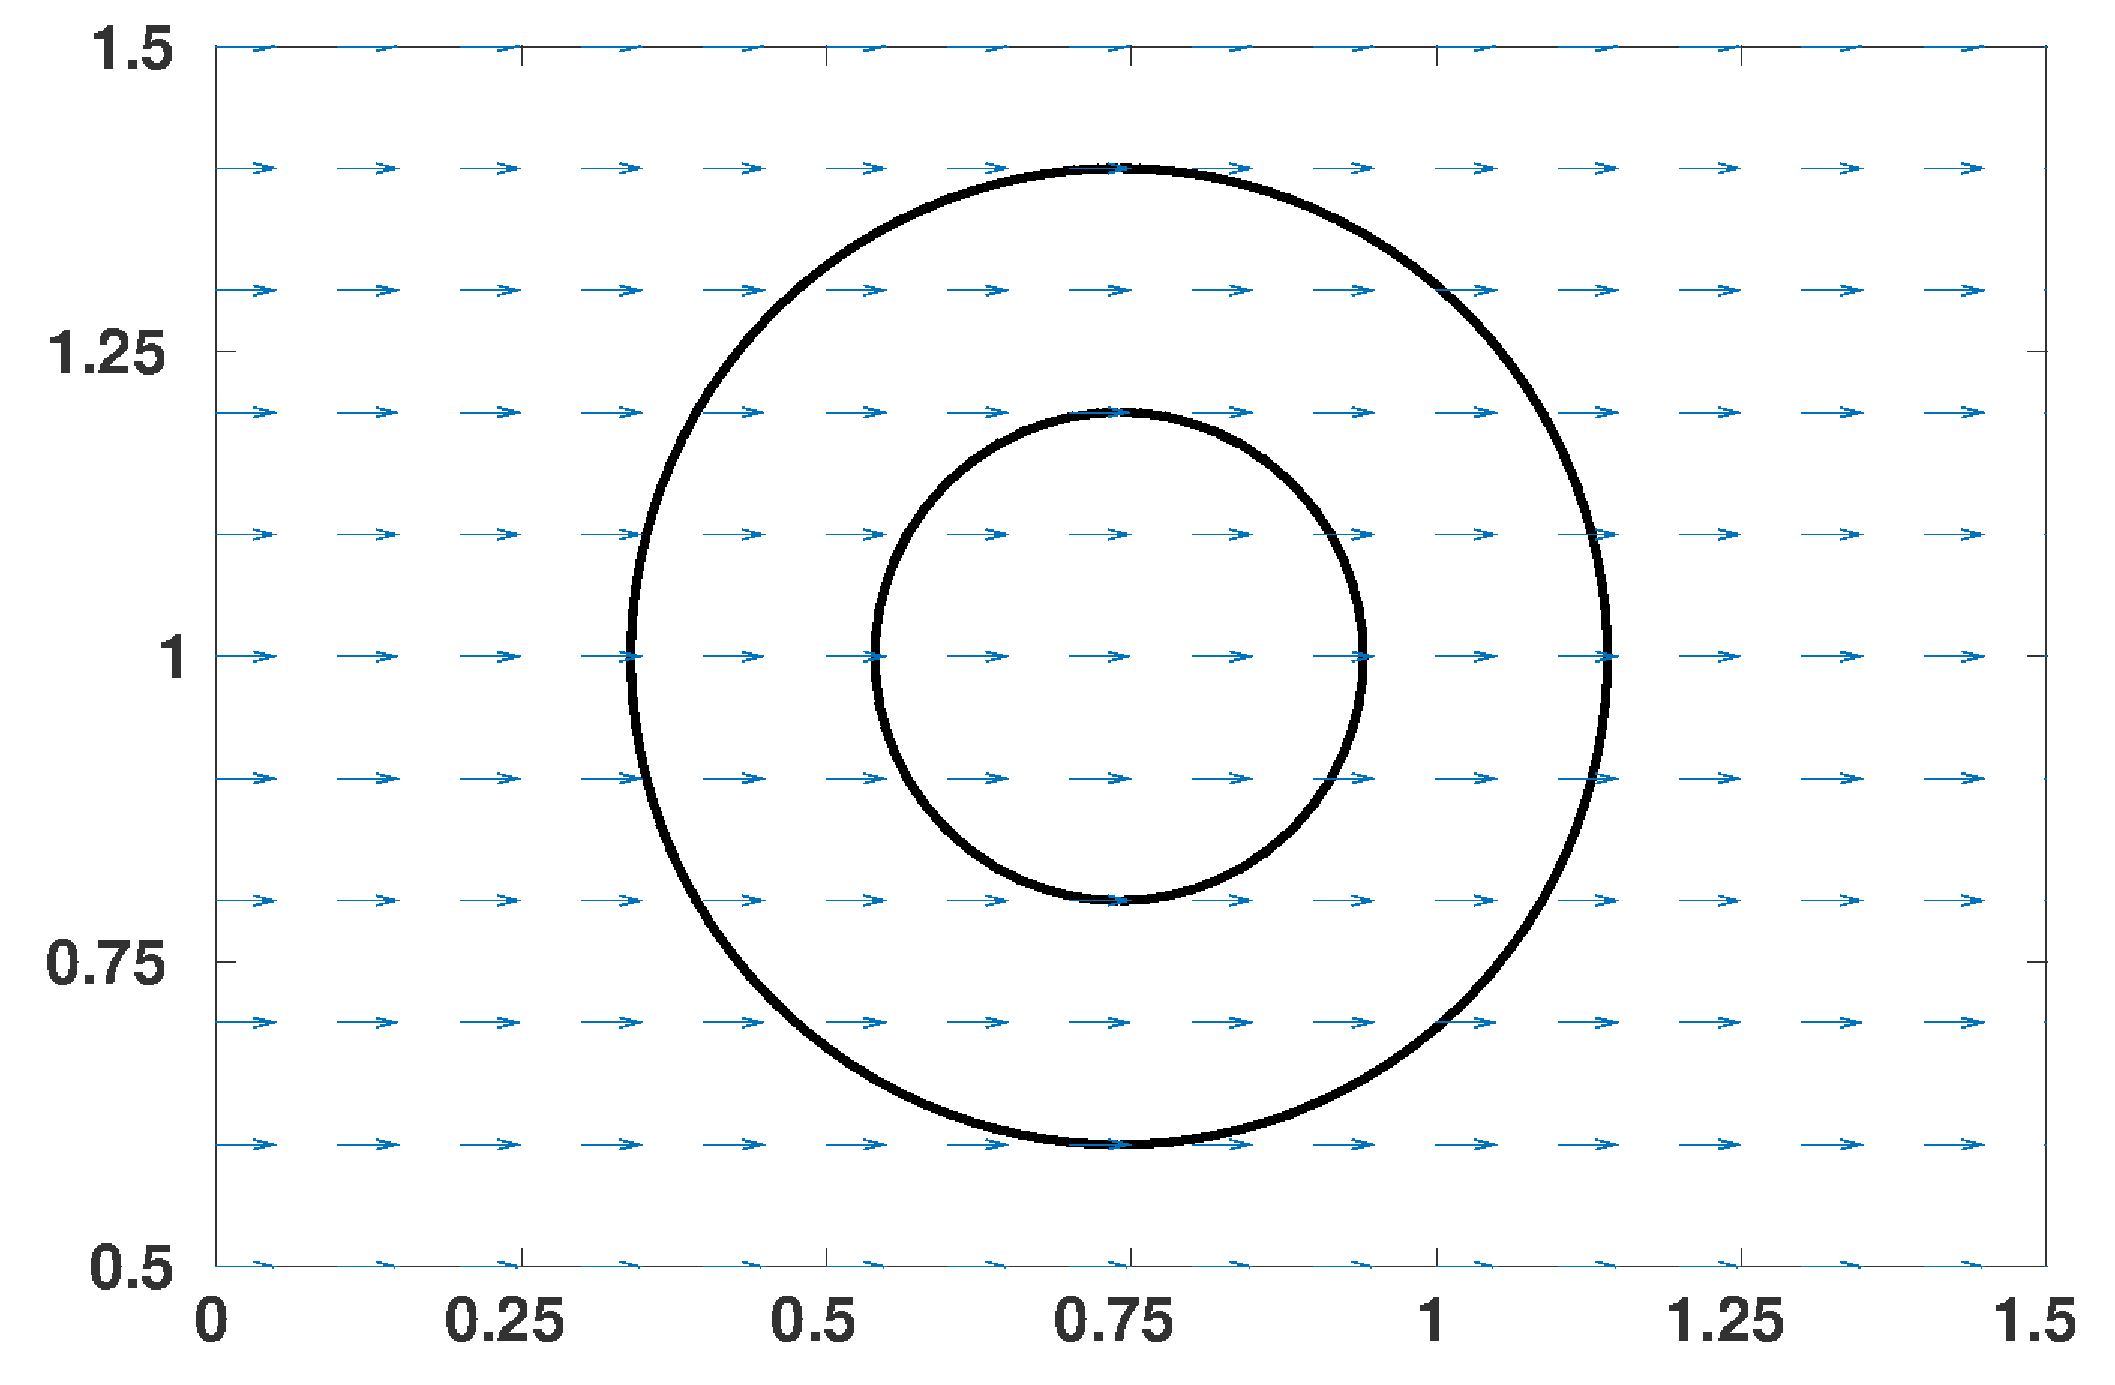
\includegraphics[width=0.5\textwidth]{IC.eps}
      }
  \subfloat[After advecting 500 steps\label{subfig-1:dummy}]{%
      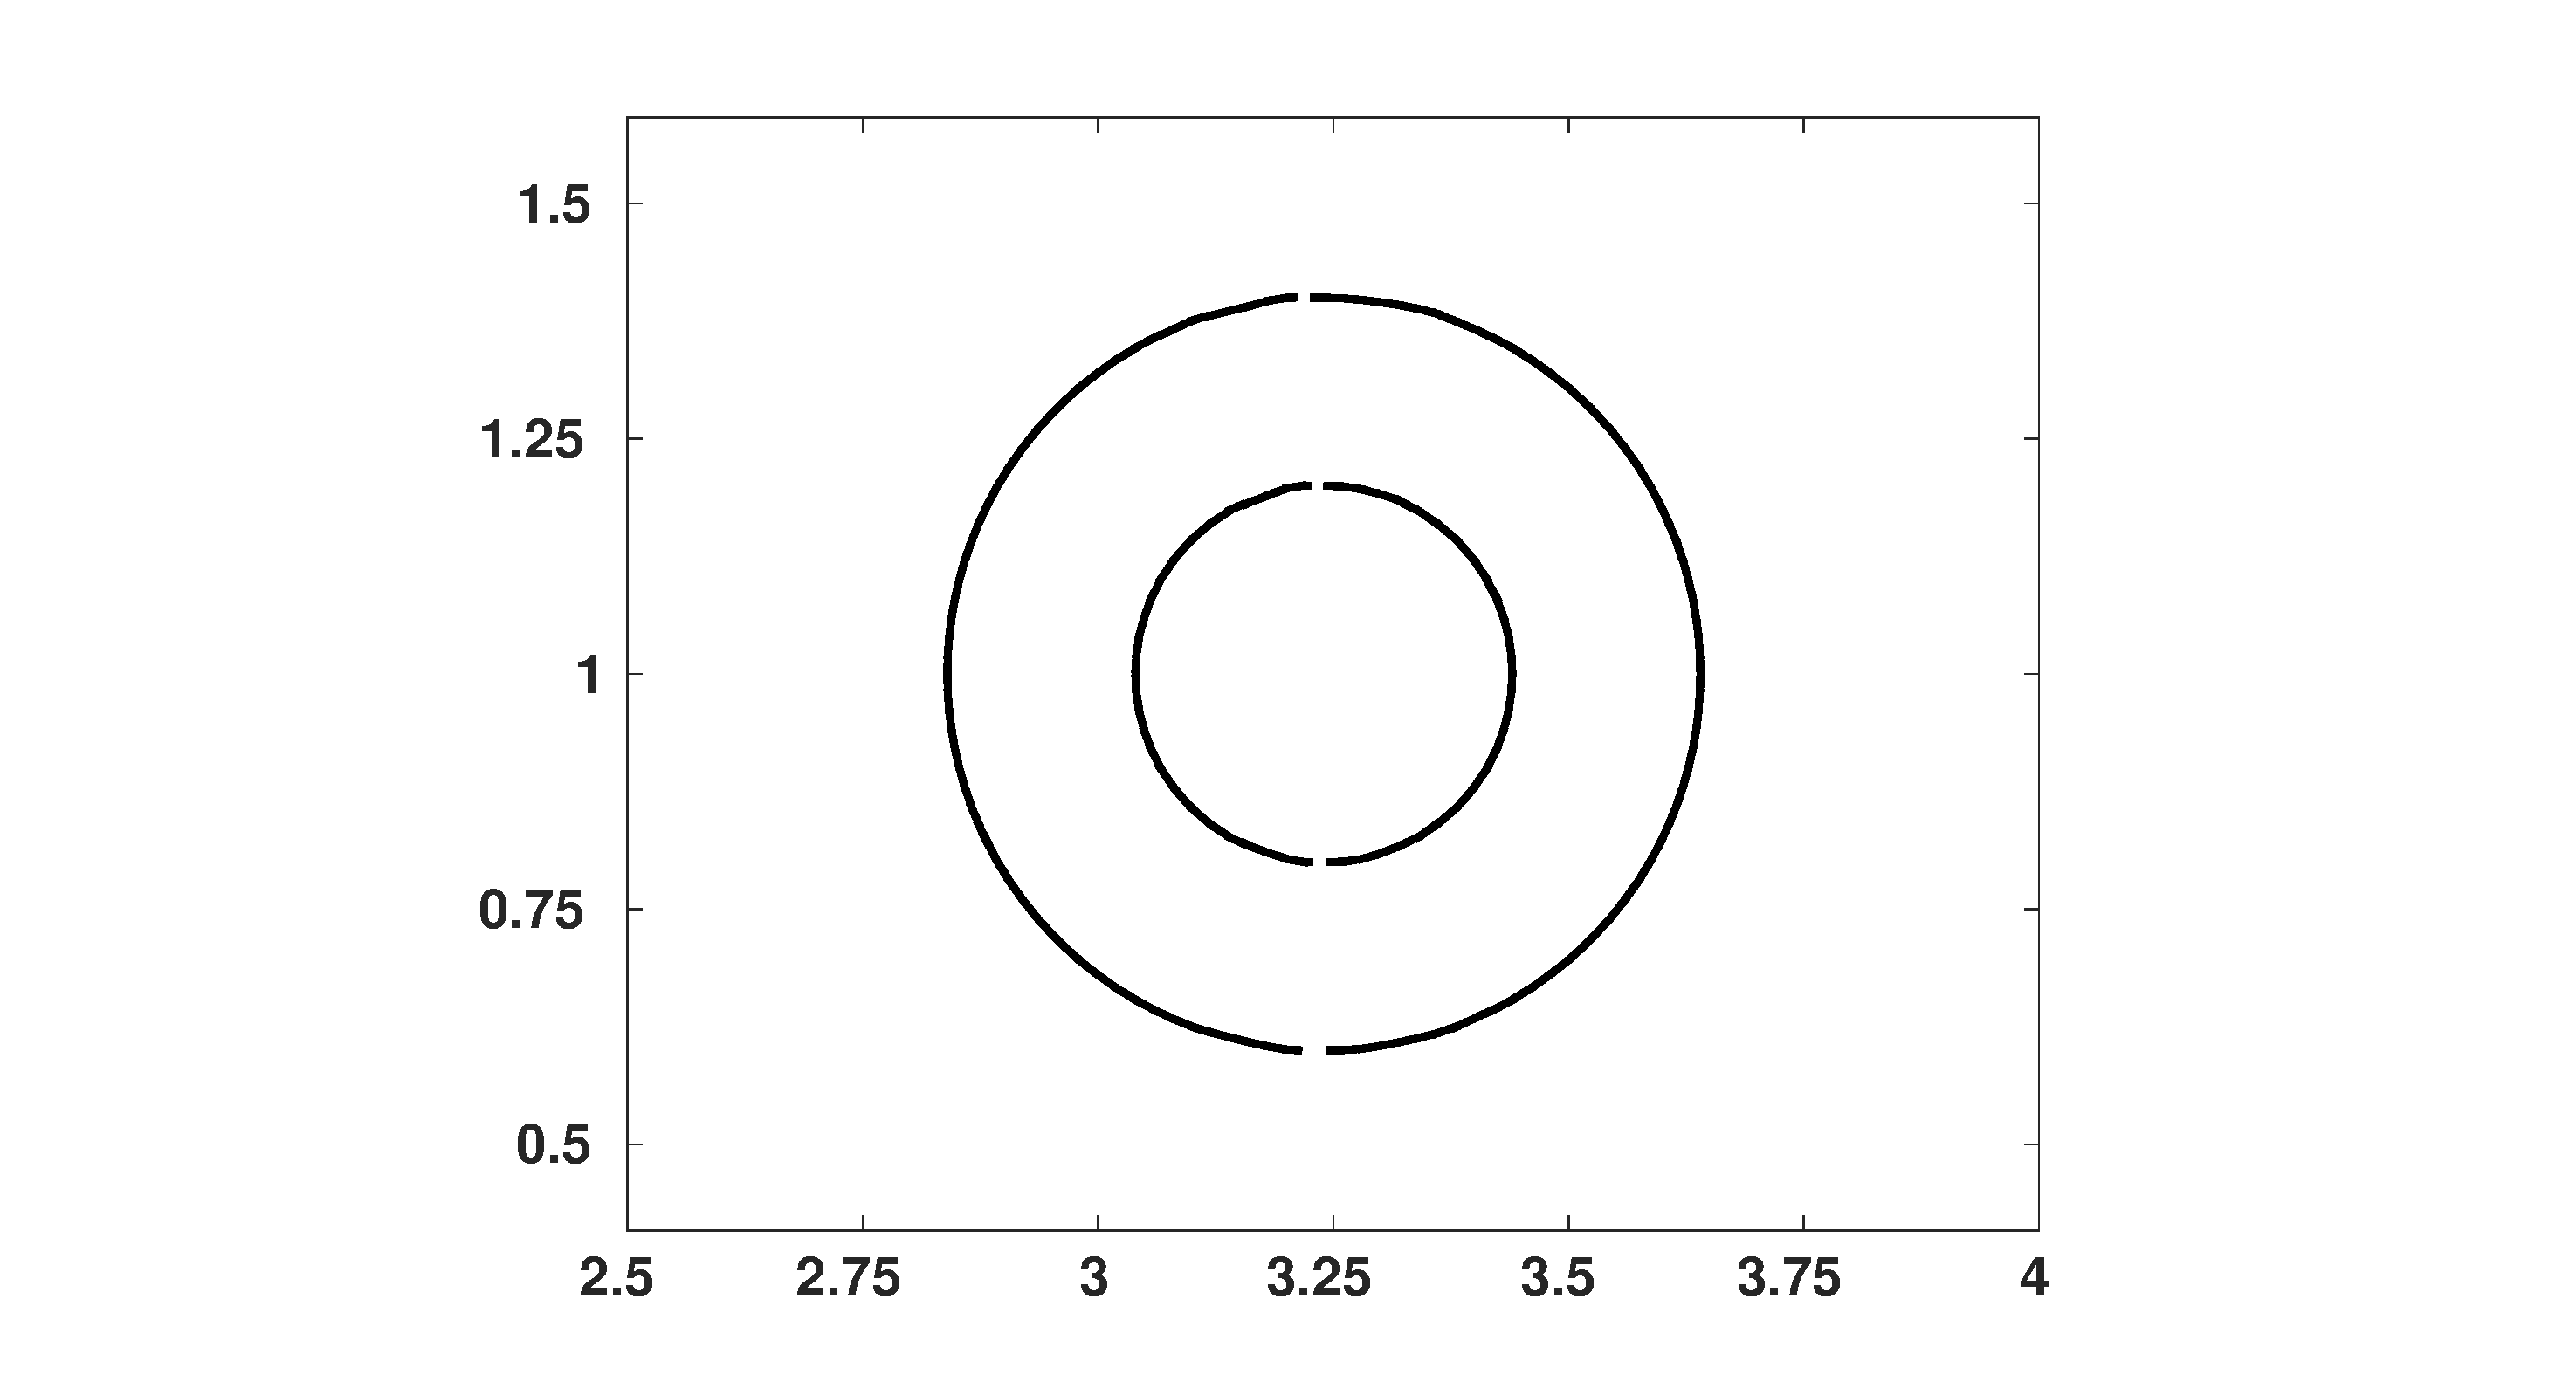
\includegraphics[width=0.5\textwidth]{final500.eps}
      }
 \caption{Advection test for velocity field U(1,0)}
\end{figure}

\begin{figure}[H]
 \centering
%  \begin{subfigure}[p]{1.0\textwidth}
%  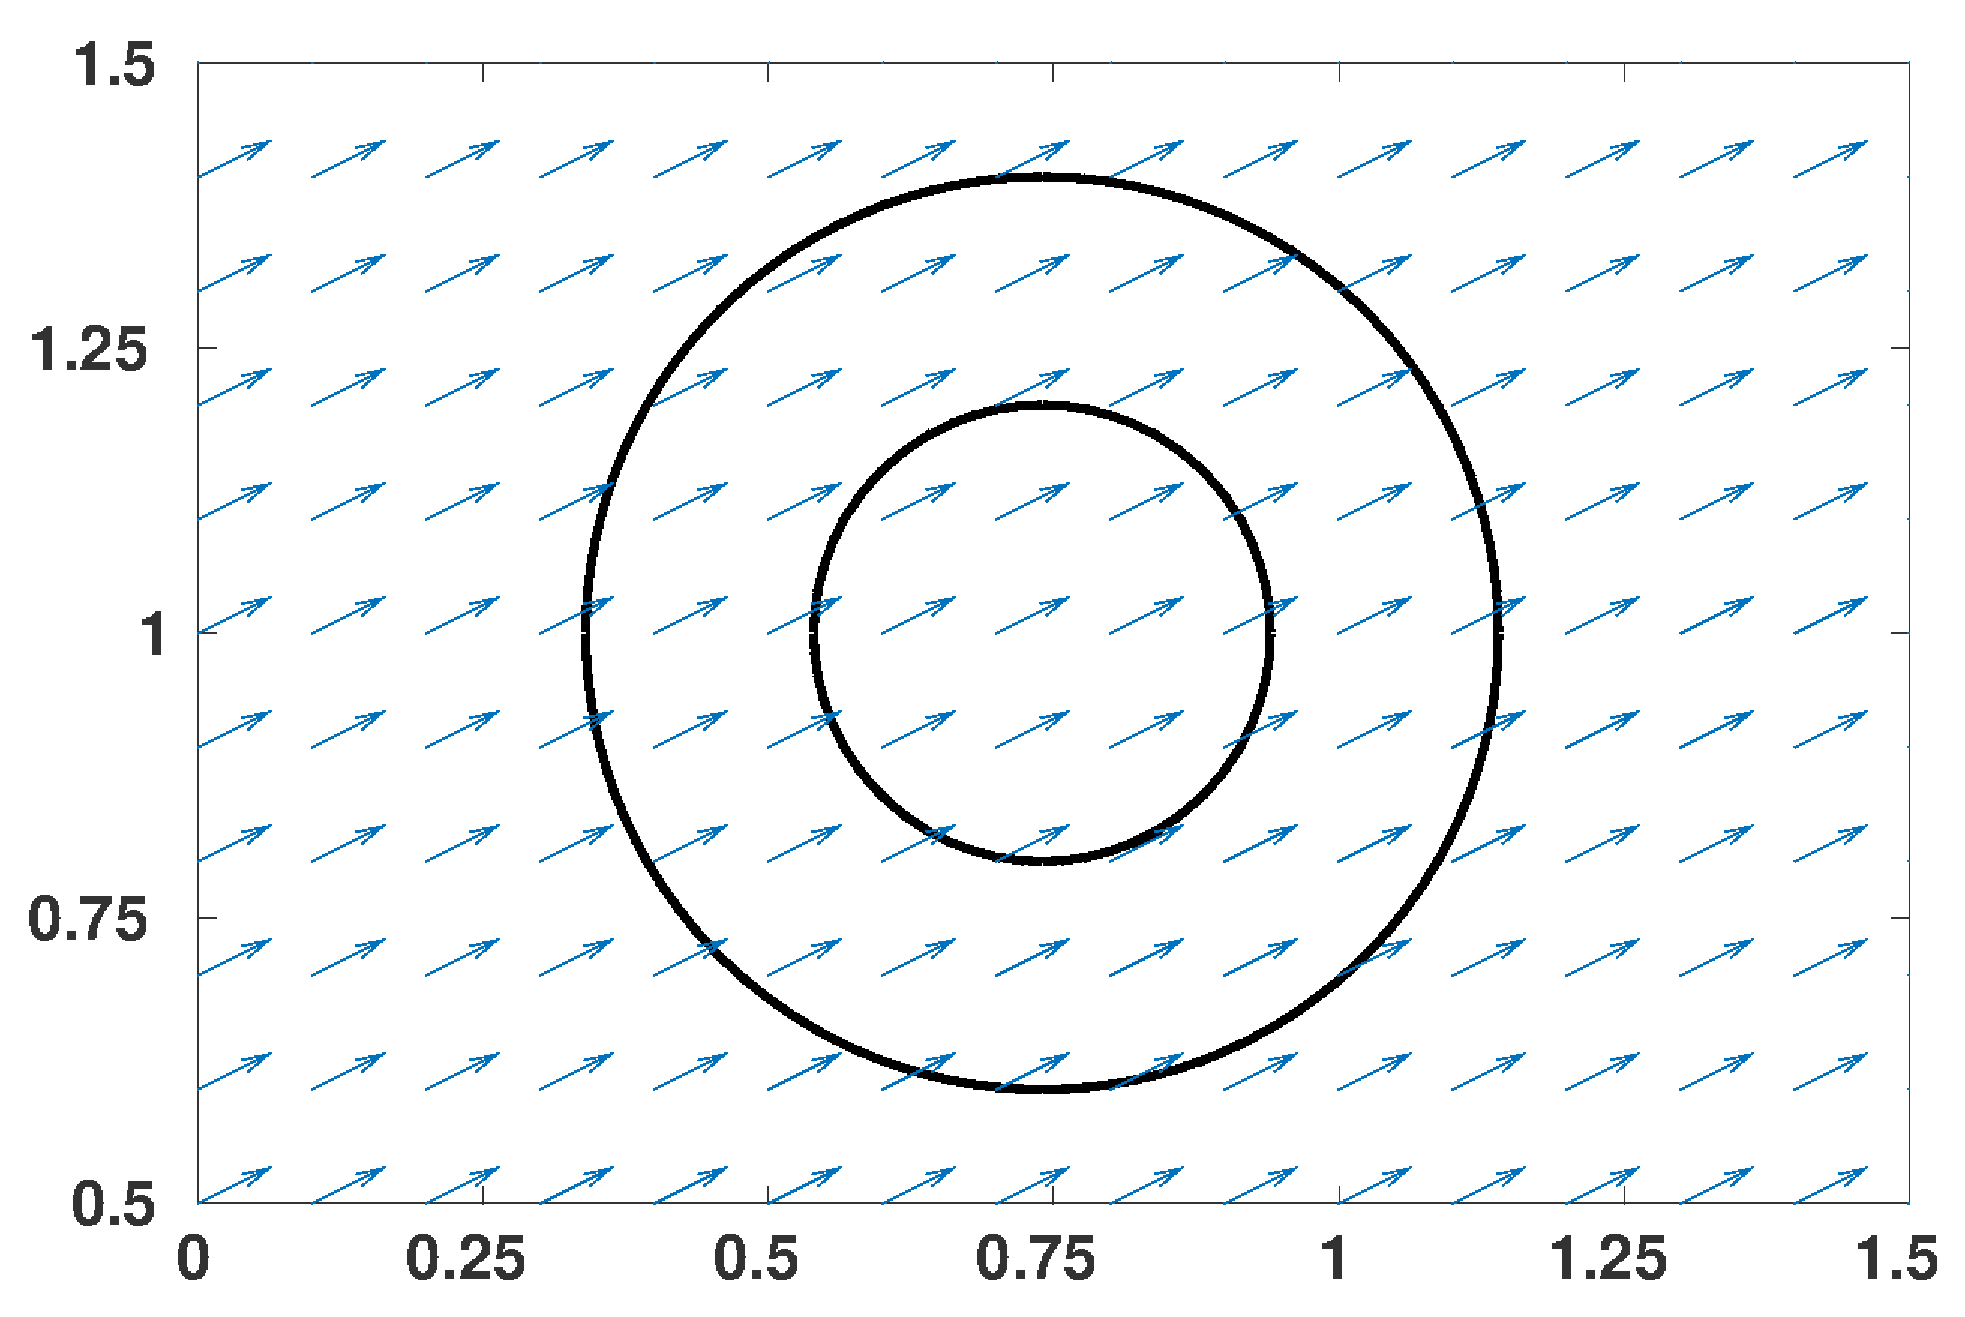
\includegraphics[width=\textwidth]{IC21.eps}
%  \caption{Initial Condition for translational test}
%  \end{subfigure}
%   \begin{subfigure}[p]{1.0\textwidth}
%  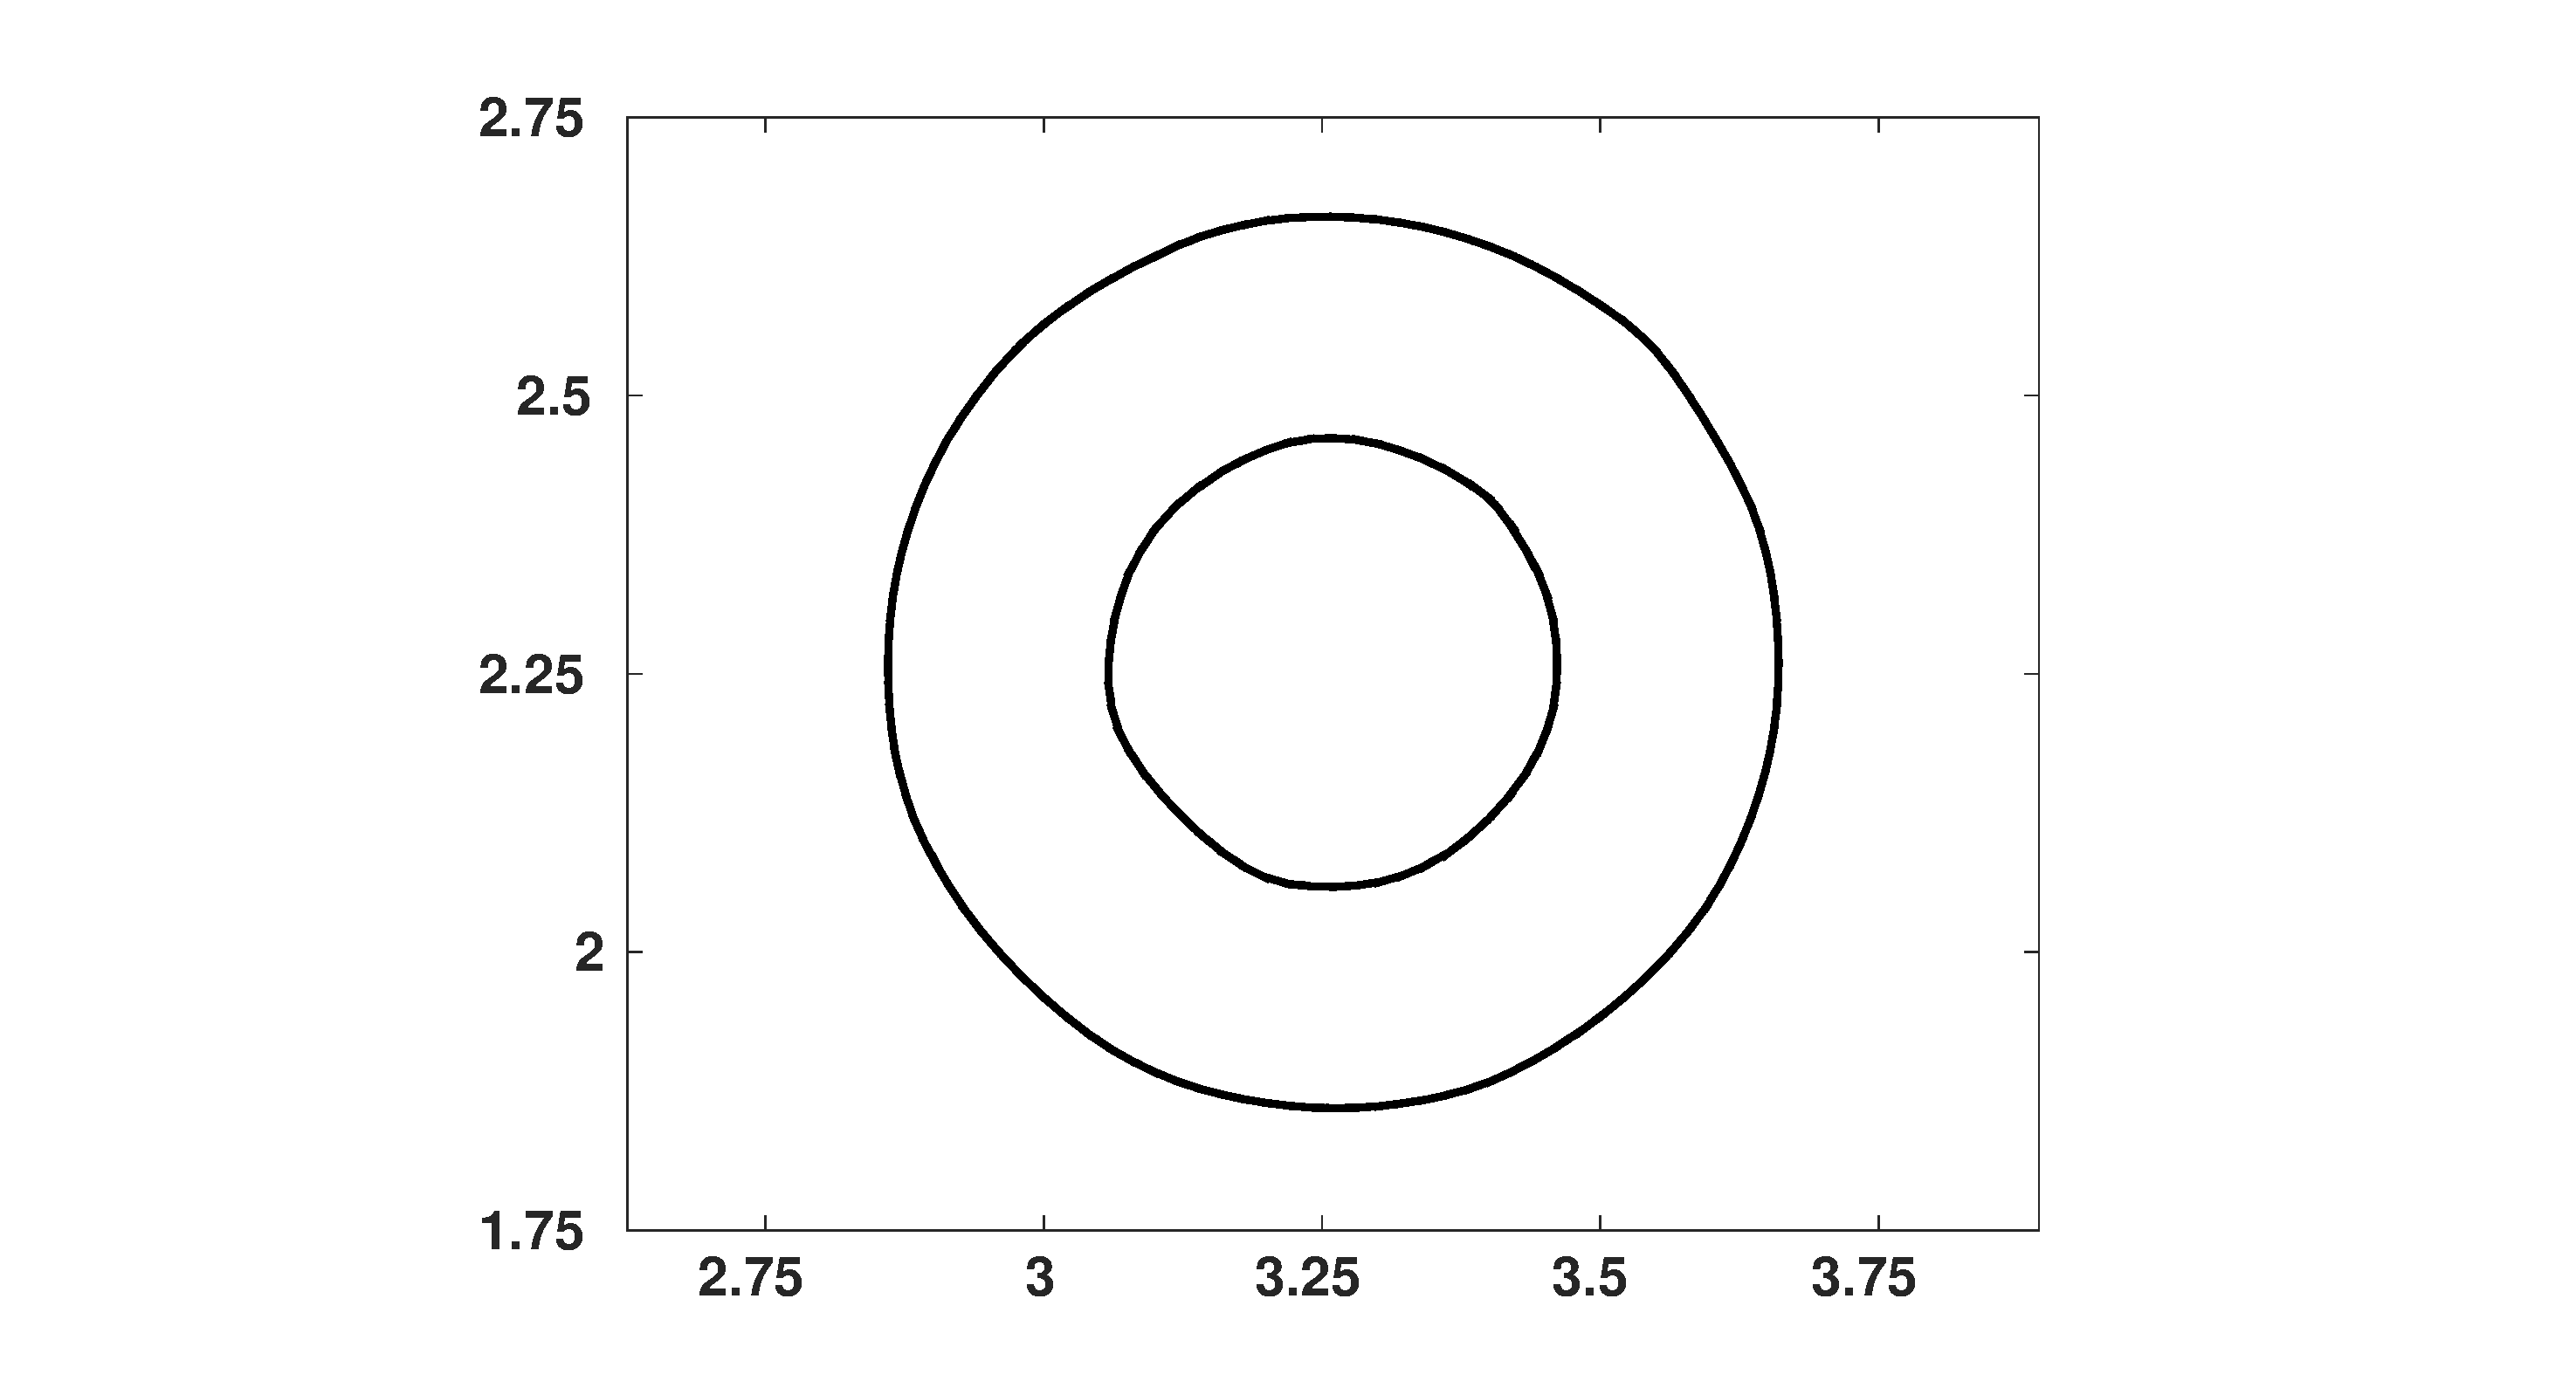
\includegraphics[width=\textwidth]{final504.eps}
%  \caption{After advecting 504 steps}
%  \end{subfigure}
 \subfloat[Initial Condition for translational test\label{subfig-1:dummy}]{%
      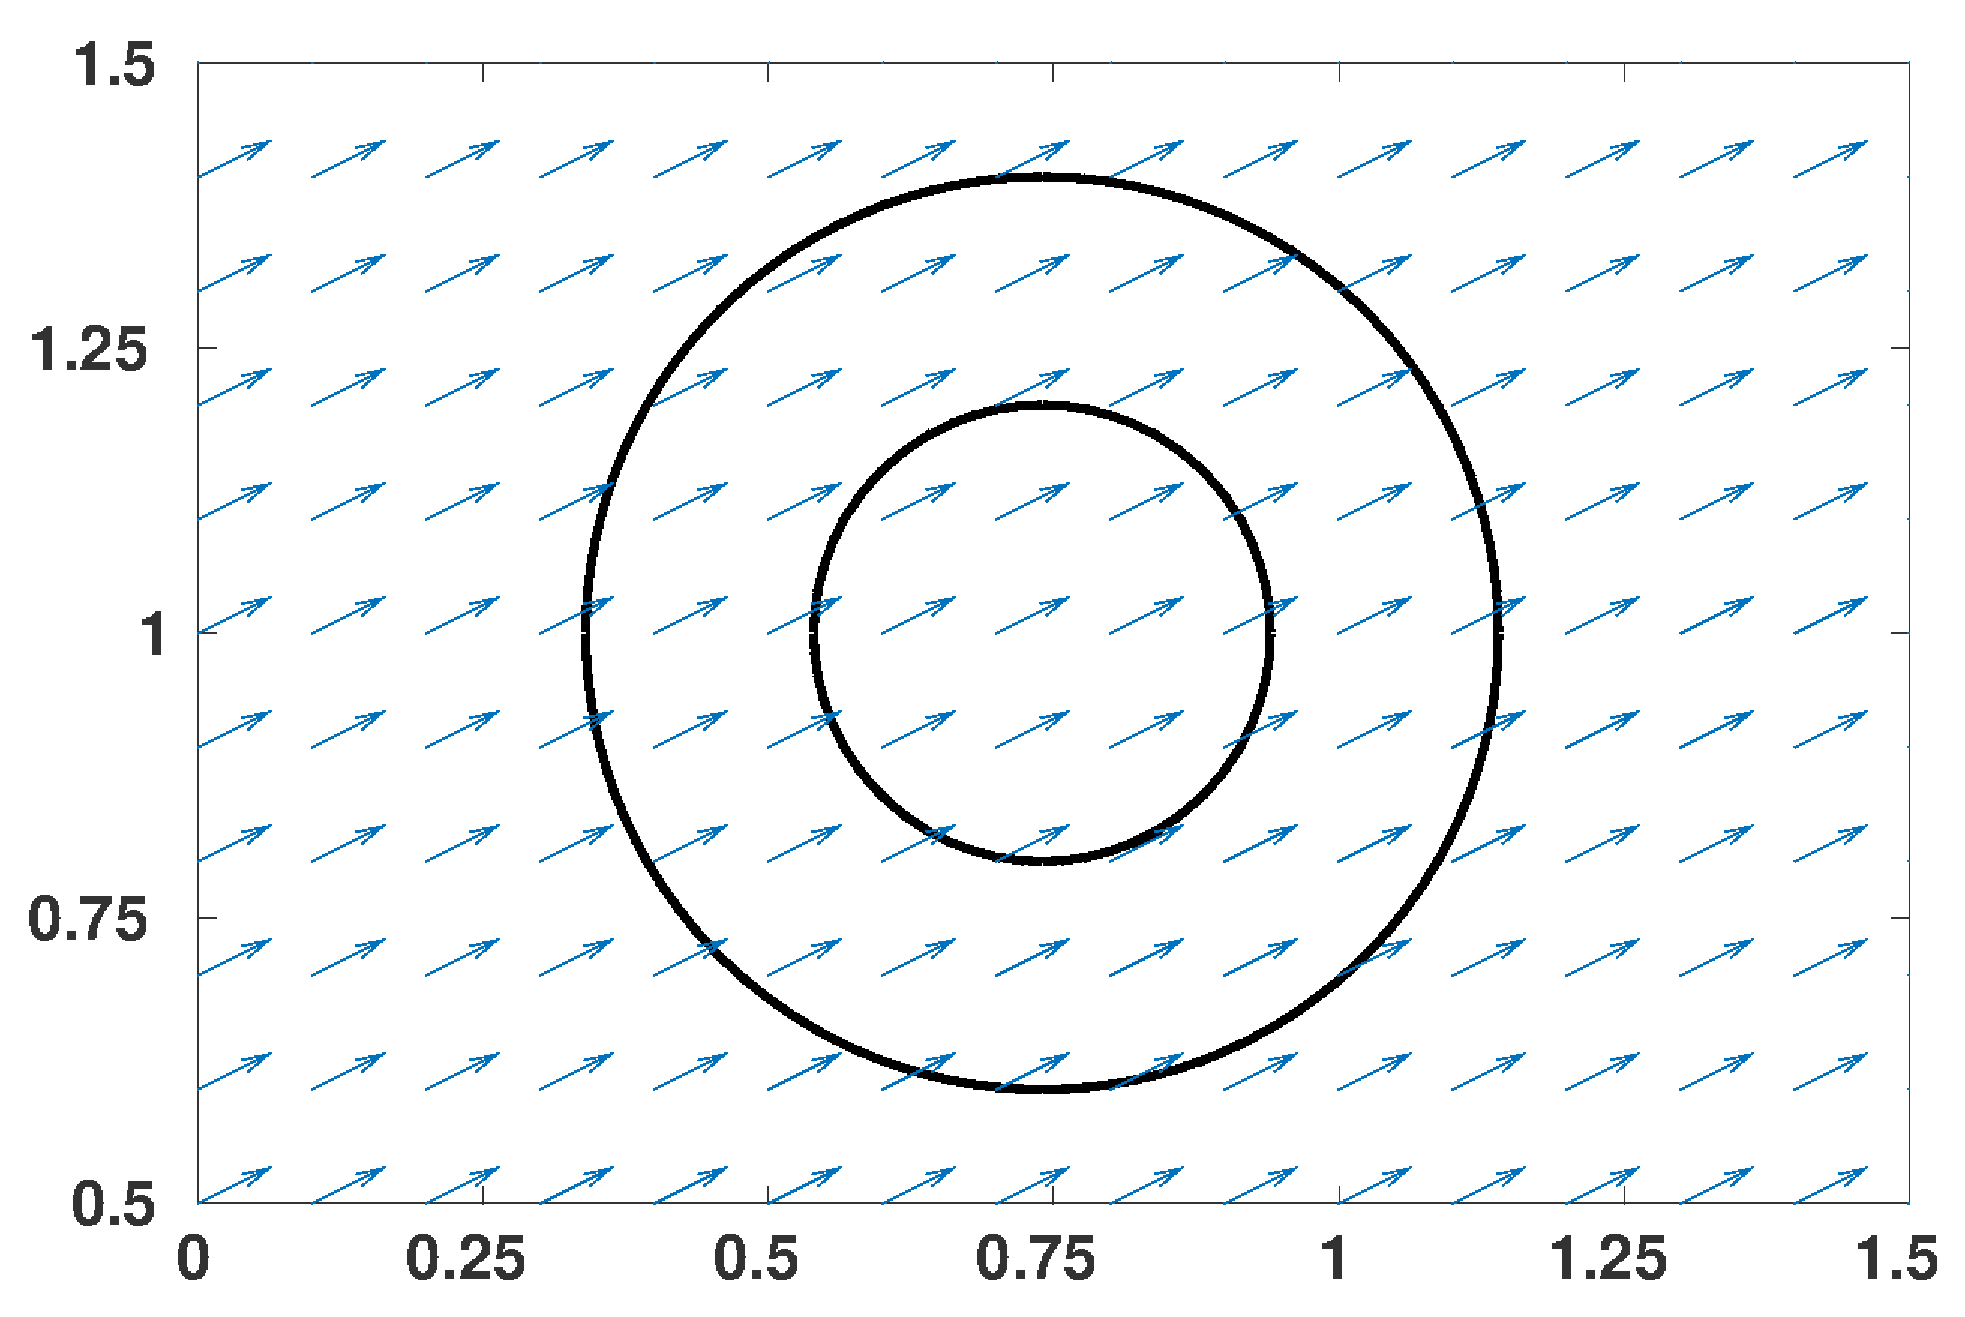
\includegraphics[width=0.5\textwidth]{IC21.eps}
      }
\subfloat[After advecting 504 steps\label{subfig-1:dummy}]{%
      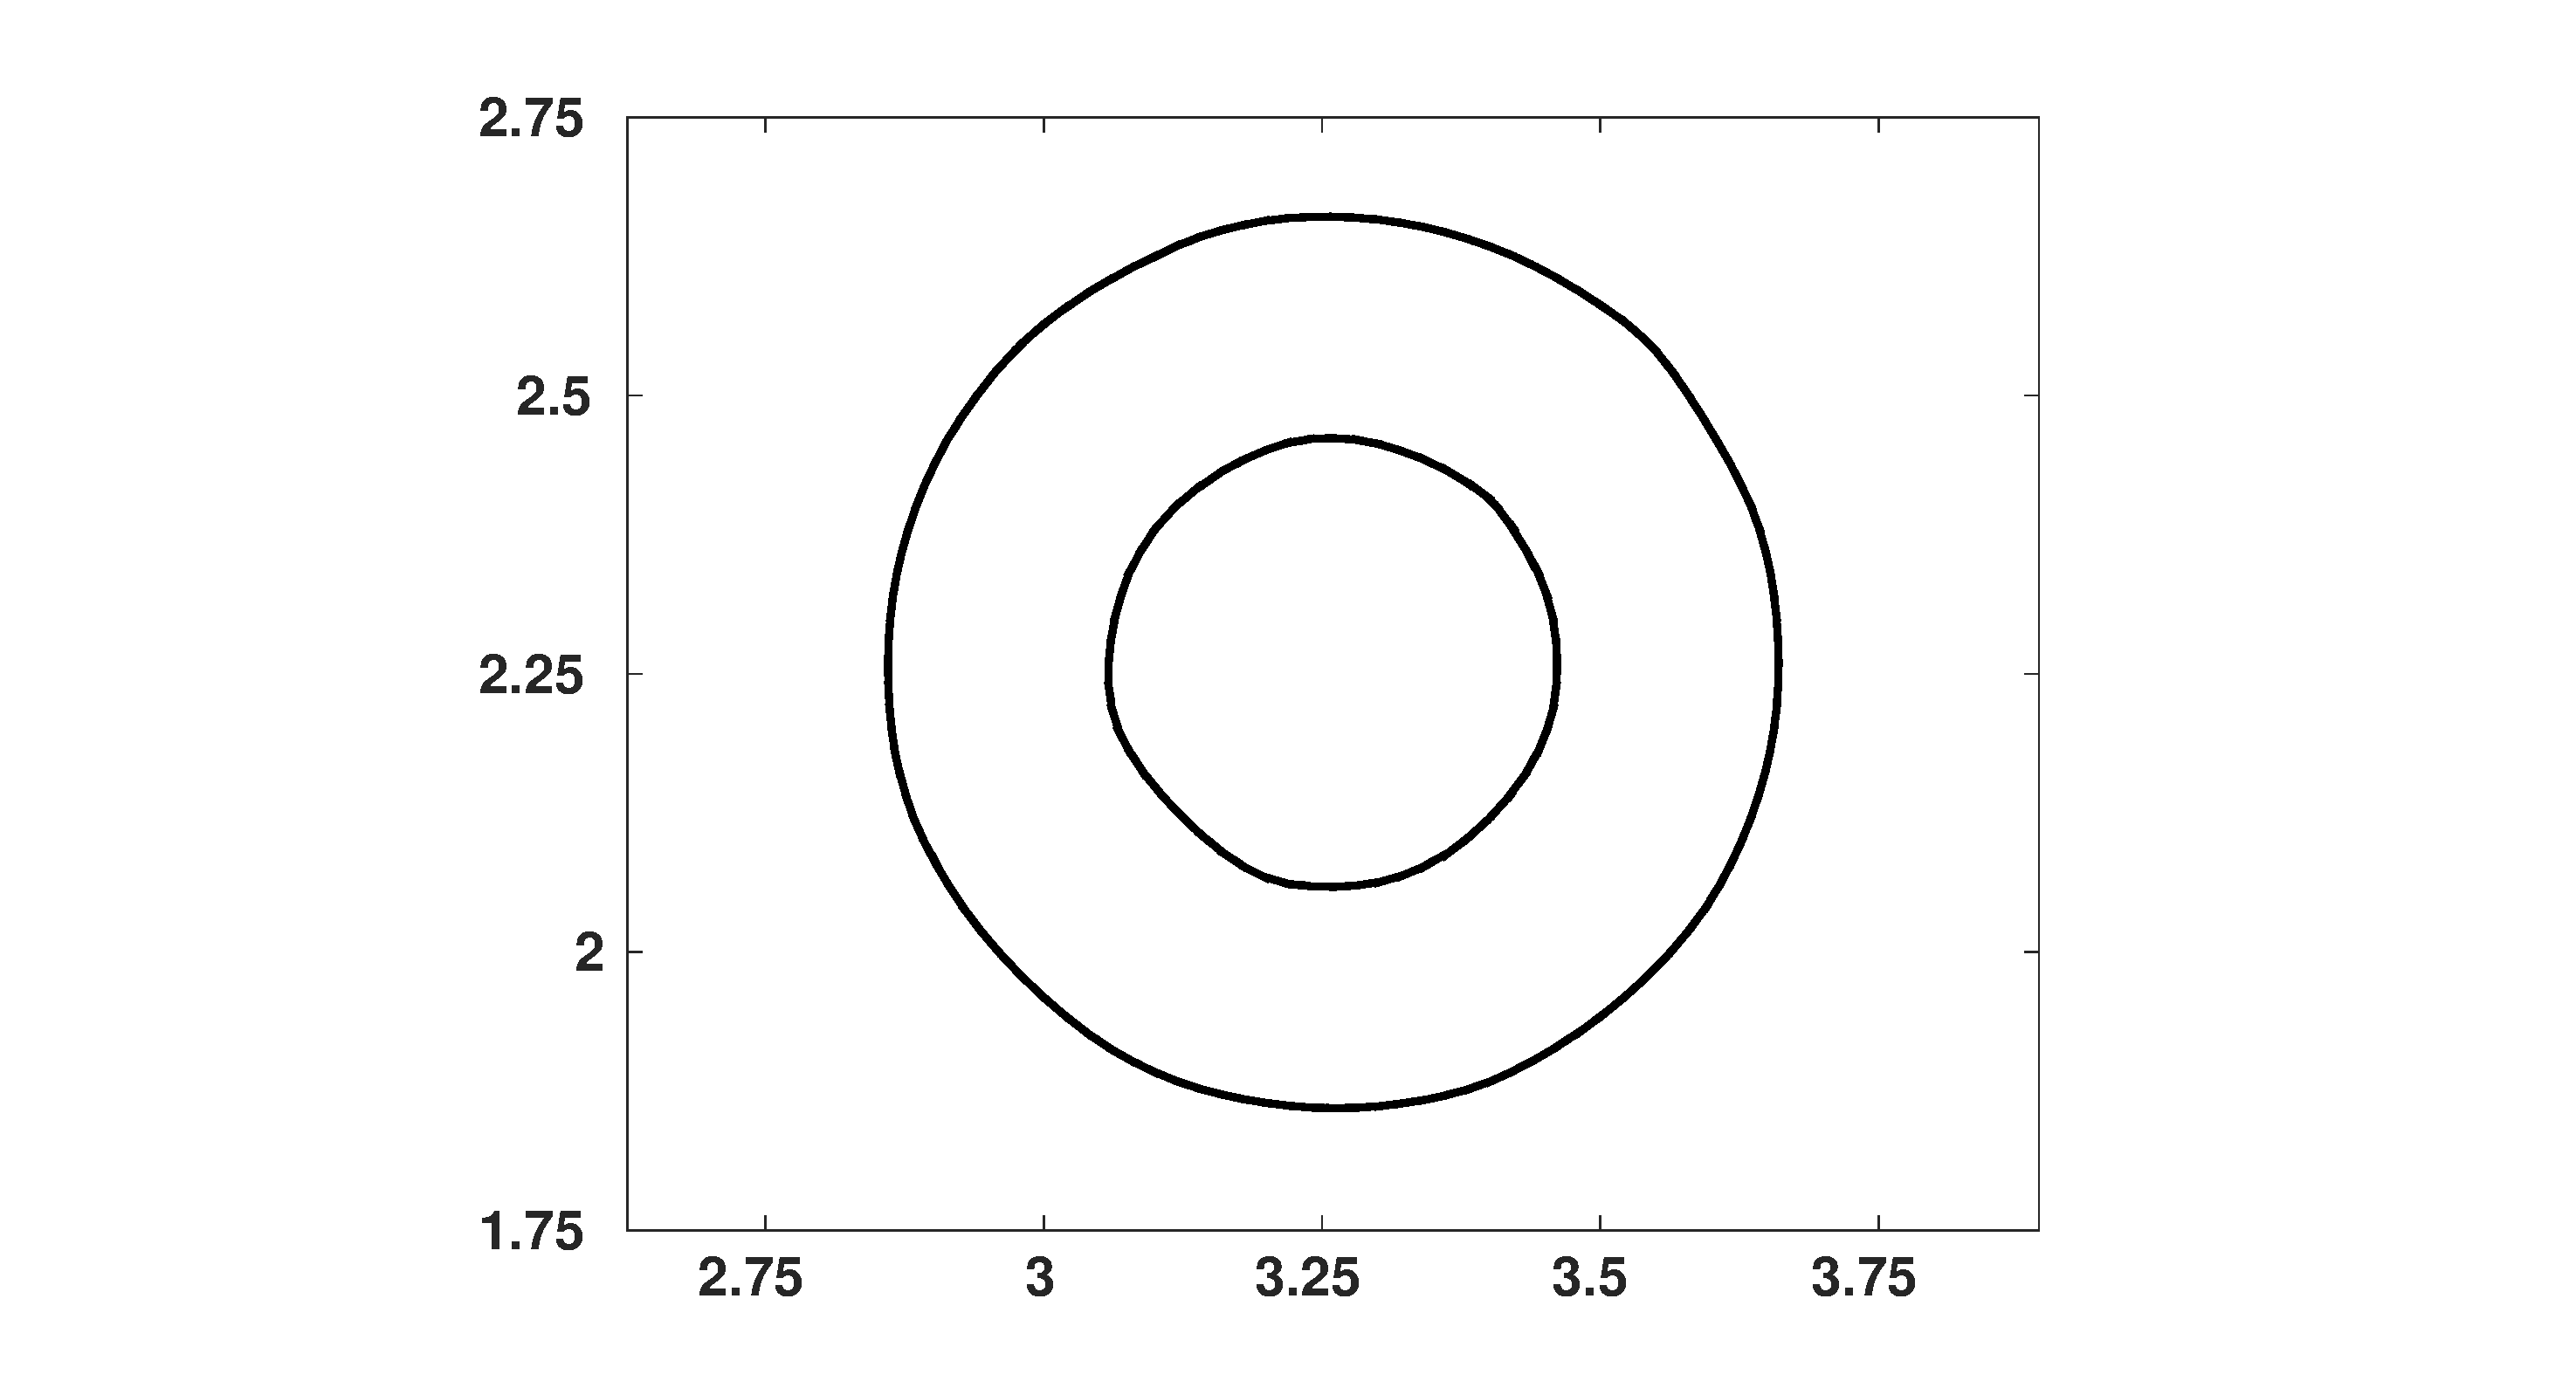
\includegraphics[width=0.5\textwidth]{final504.eps}
      }
 \caption{Advection test for velocity field U(2,1)}
\end{figure}

\subsection{Advection test for solid body rotation}
For solid body rotation test a slotted circle configuration is taken from \cite{Zalesak1979}, the center of slotted circle is at
(2.0,2.75) and diameter is 1.0. The length and width of slot is 0.6 and 0.12 respectively.(Fig. 3(a))  The refinement of the domain which is $4.0X4.0$ is $200X200$.
A curl free velocity field is given by $U(-\Omega(y-y_0),\Omega(x-x_0))$, where axis of rotation passes through the $(x_0,y_0)$ and normal to the x-y plane. $\Omega$ is 
the angular velocity. Here $\Omega = 0.5$ and $(x_0,y_0)$ is $(2,2)$. The time step is 0.005.

   \begin{enumerate}
   \setlength\itemsep{1em}
 \item Domain: [0,4] x [0,4]
 \item Grid Size: 200 x 200
 \item Radius of circle :0.5
 \item Center : (2.0,2.75)
 \item Velocity field:  $U(-0.5(y-2),0.5(x-2))$
 \end{enumerate}

\begin{figure}[H]
 \centering 
 \subfloat[Initial Condition for solid body rotation test\label{subfig-1:dummy}]{%
      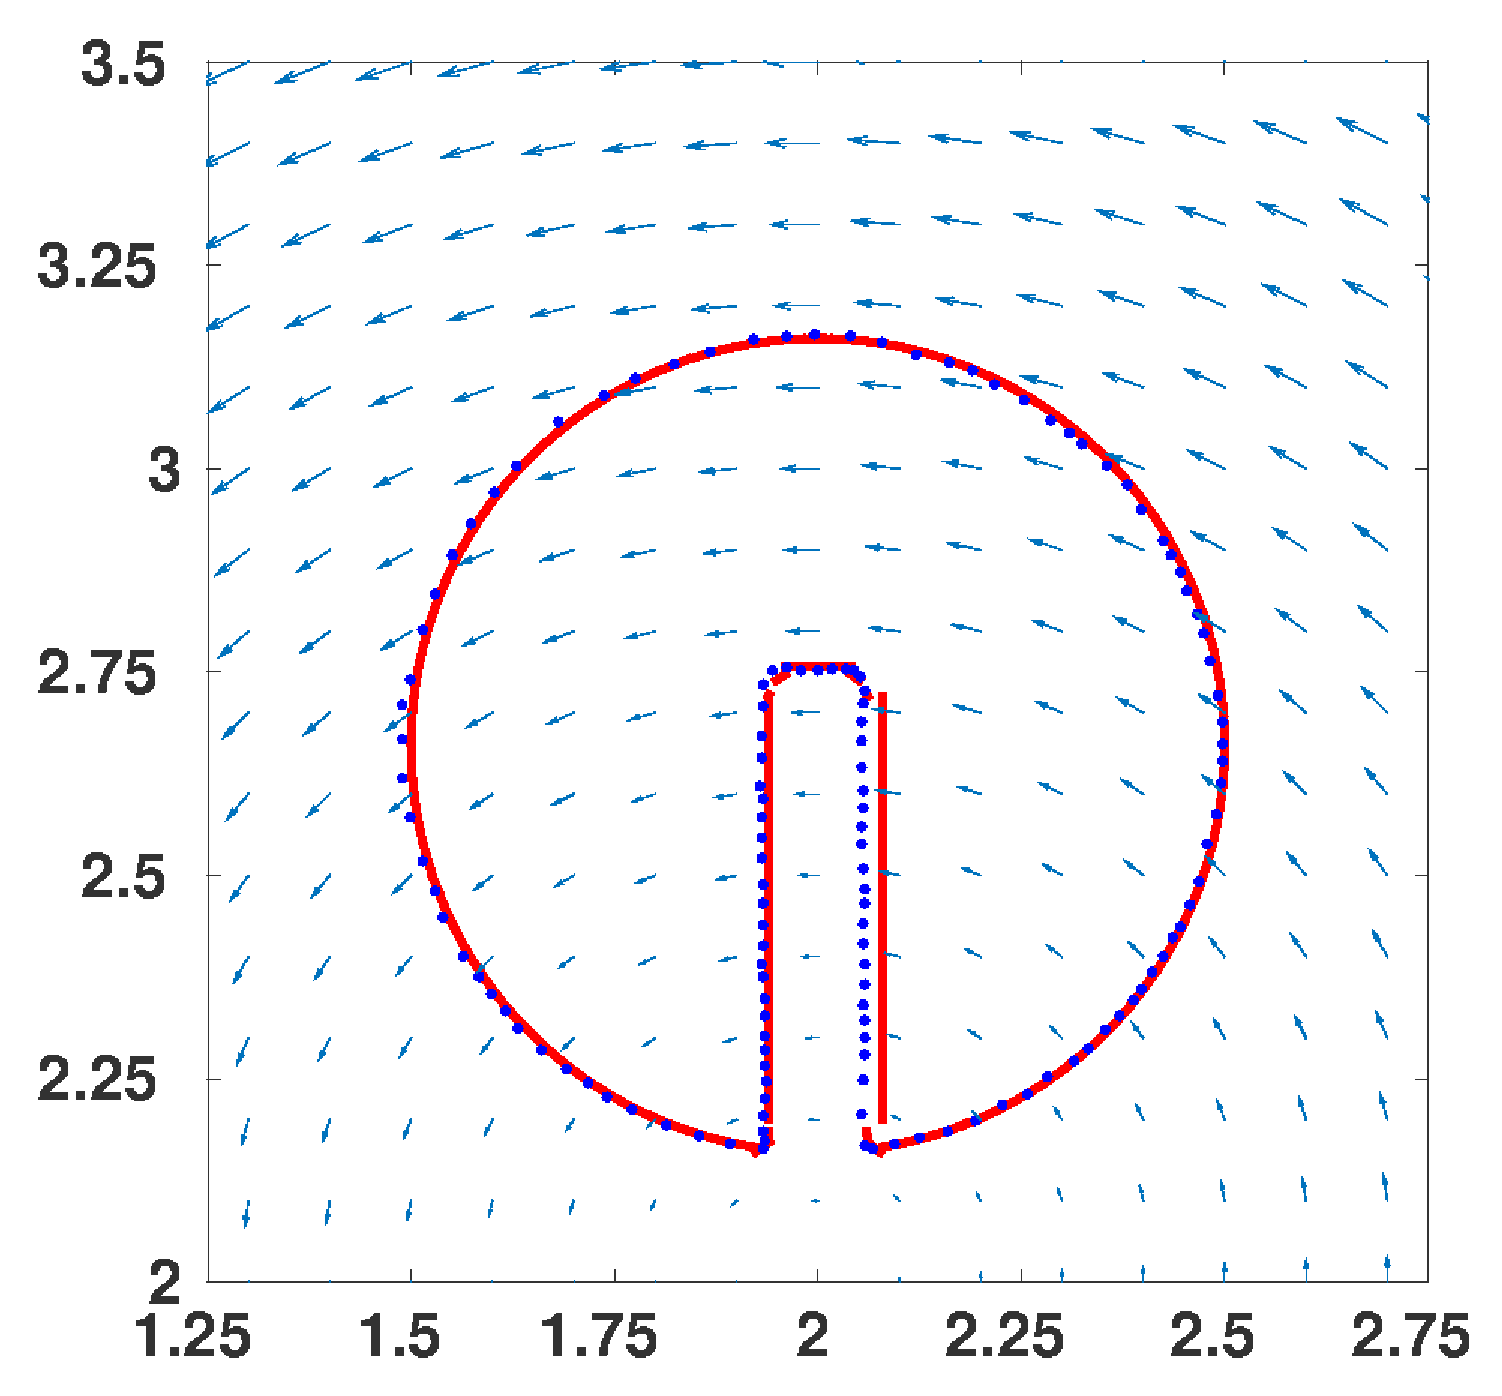
\includegraphics[width=0.8\textwidth]{SC_IC.eps}
      } \\
  \subfloat[After one full rotation\label{subfig-1:dummy}]{%
      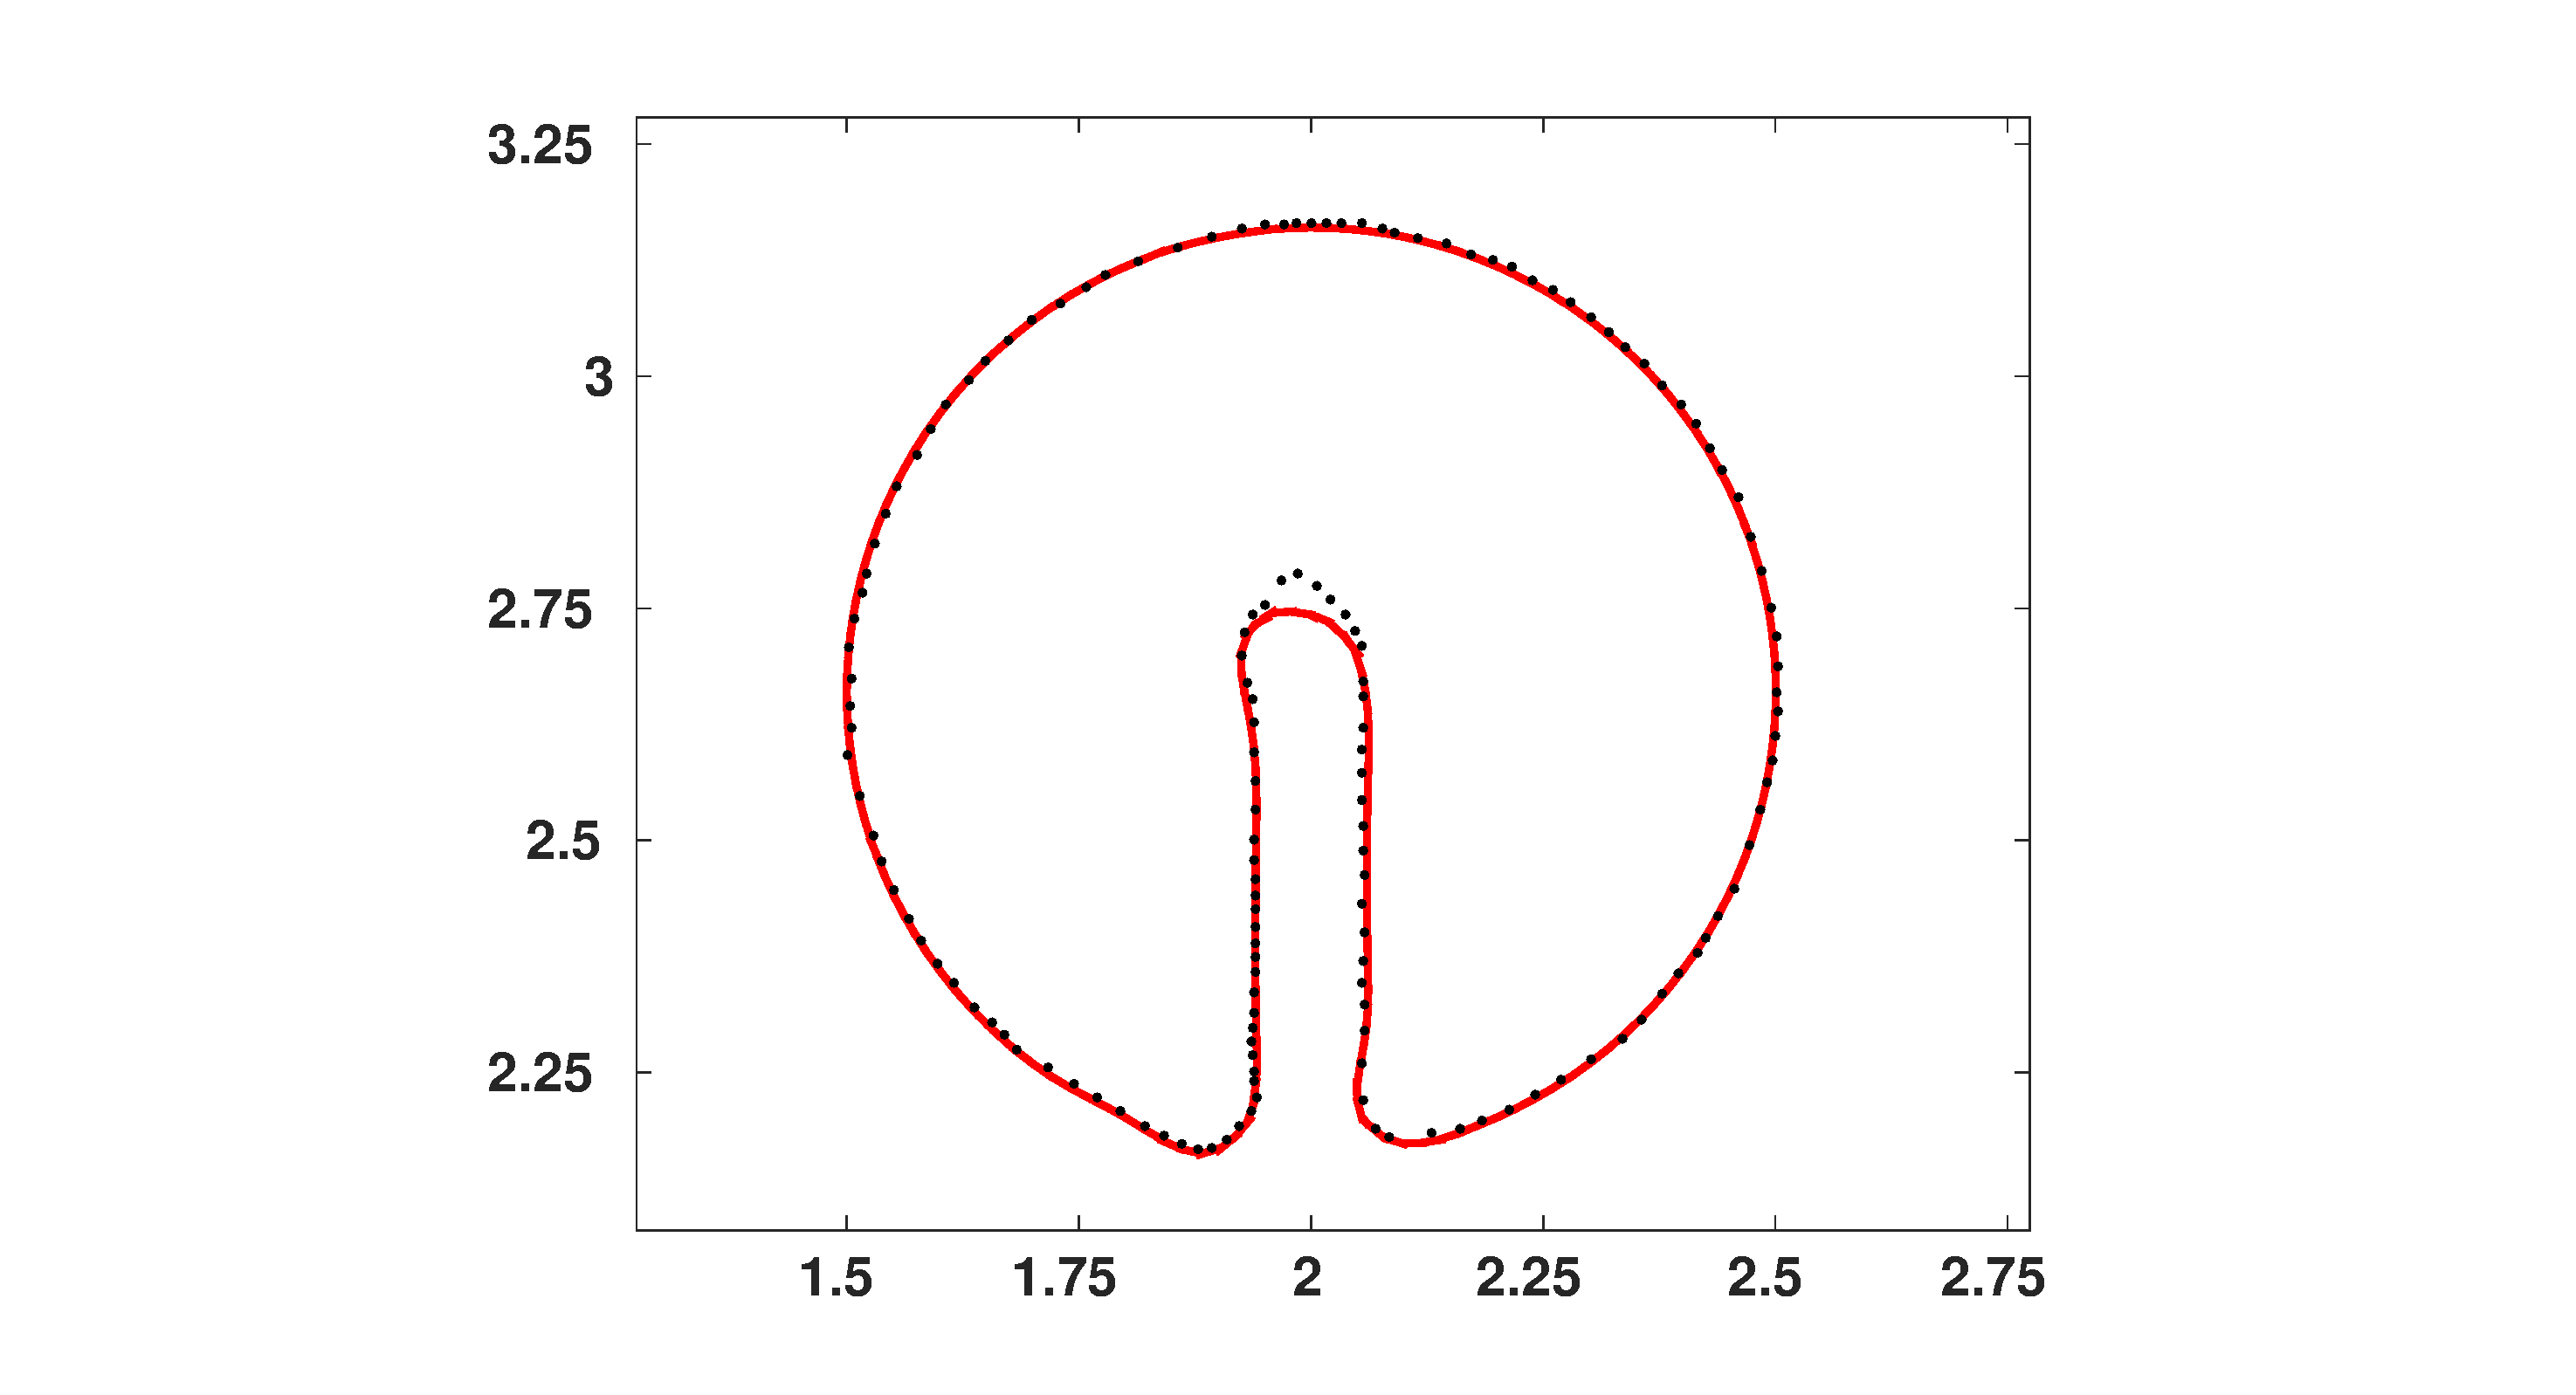
\includegraphics[width=0.8\textwidth]{SC_2513.eps}
      }
 \caption{Comparison with \cite{Rudman1997} results. (Red LVIRA and Black \cite{Rudman1997} data)}
\end{figure}
% 
\begin{figure}[H]
  \subfloat[After advecting 628 steps\label{subfig-1:dummy}]{%
      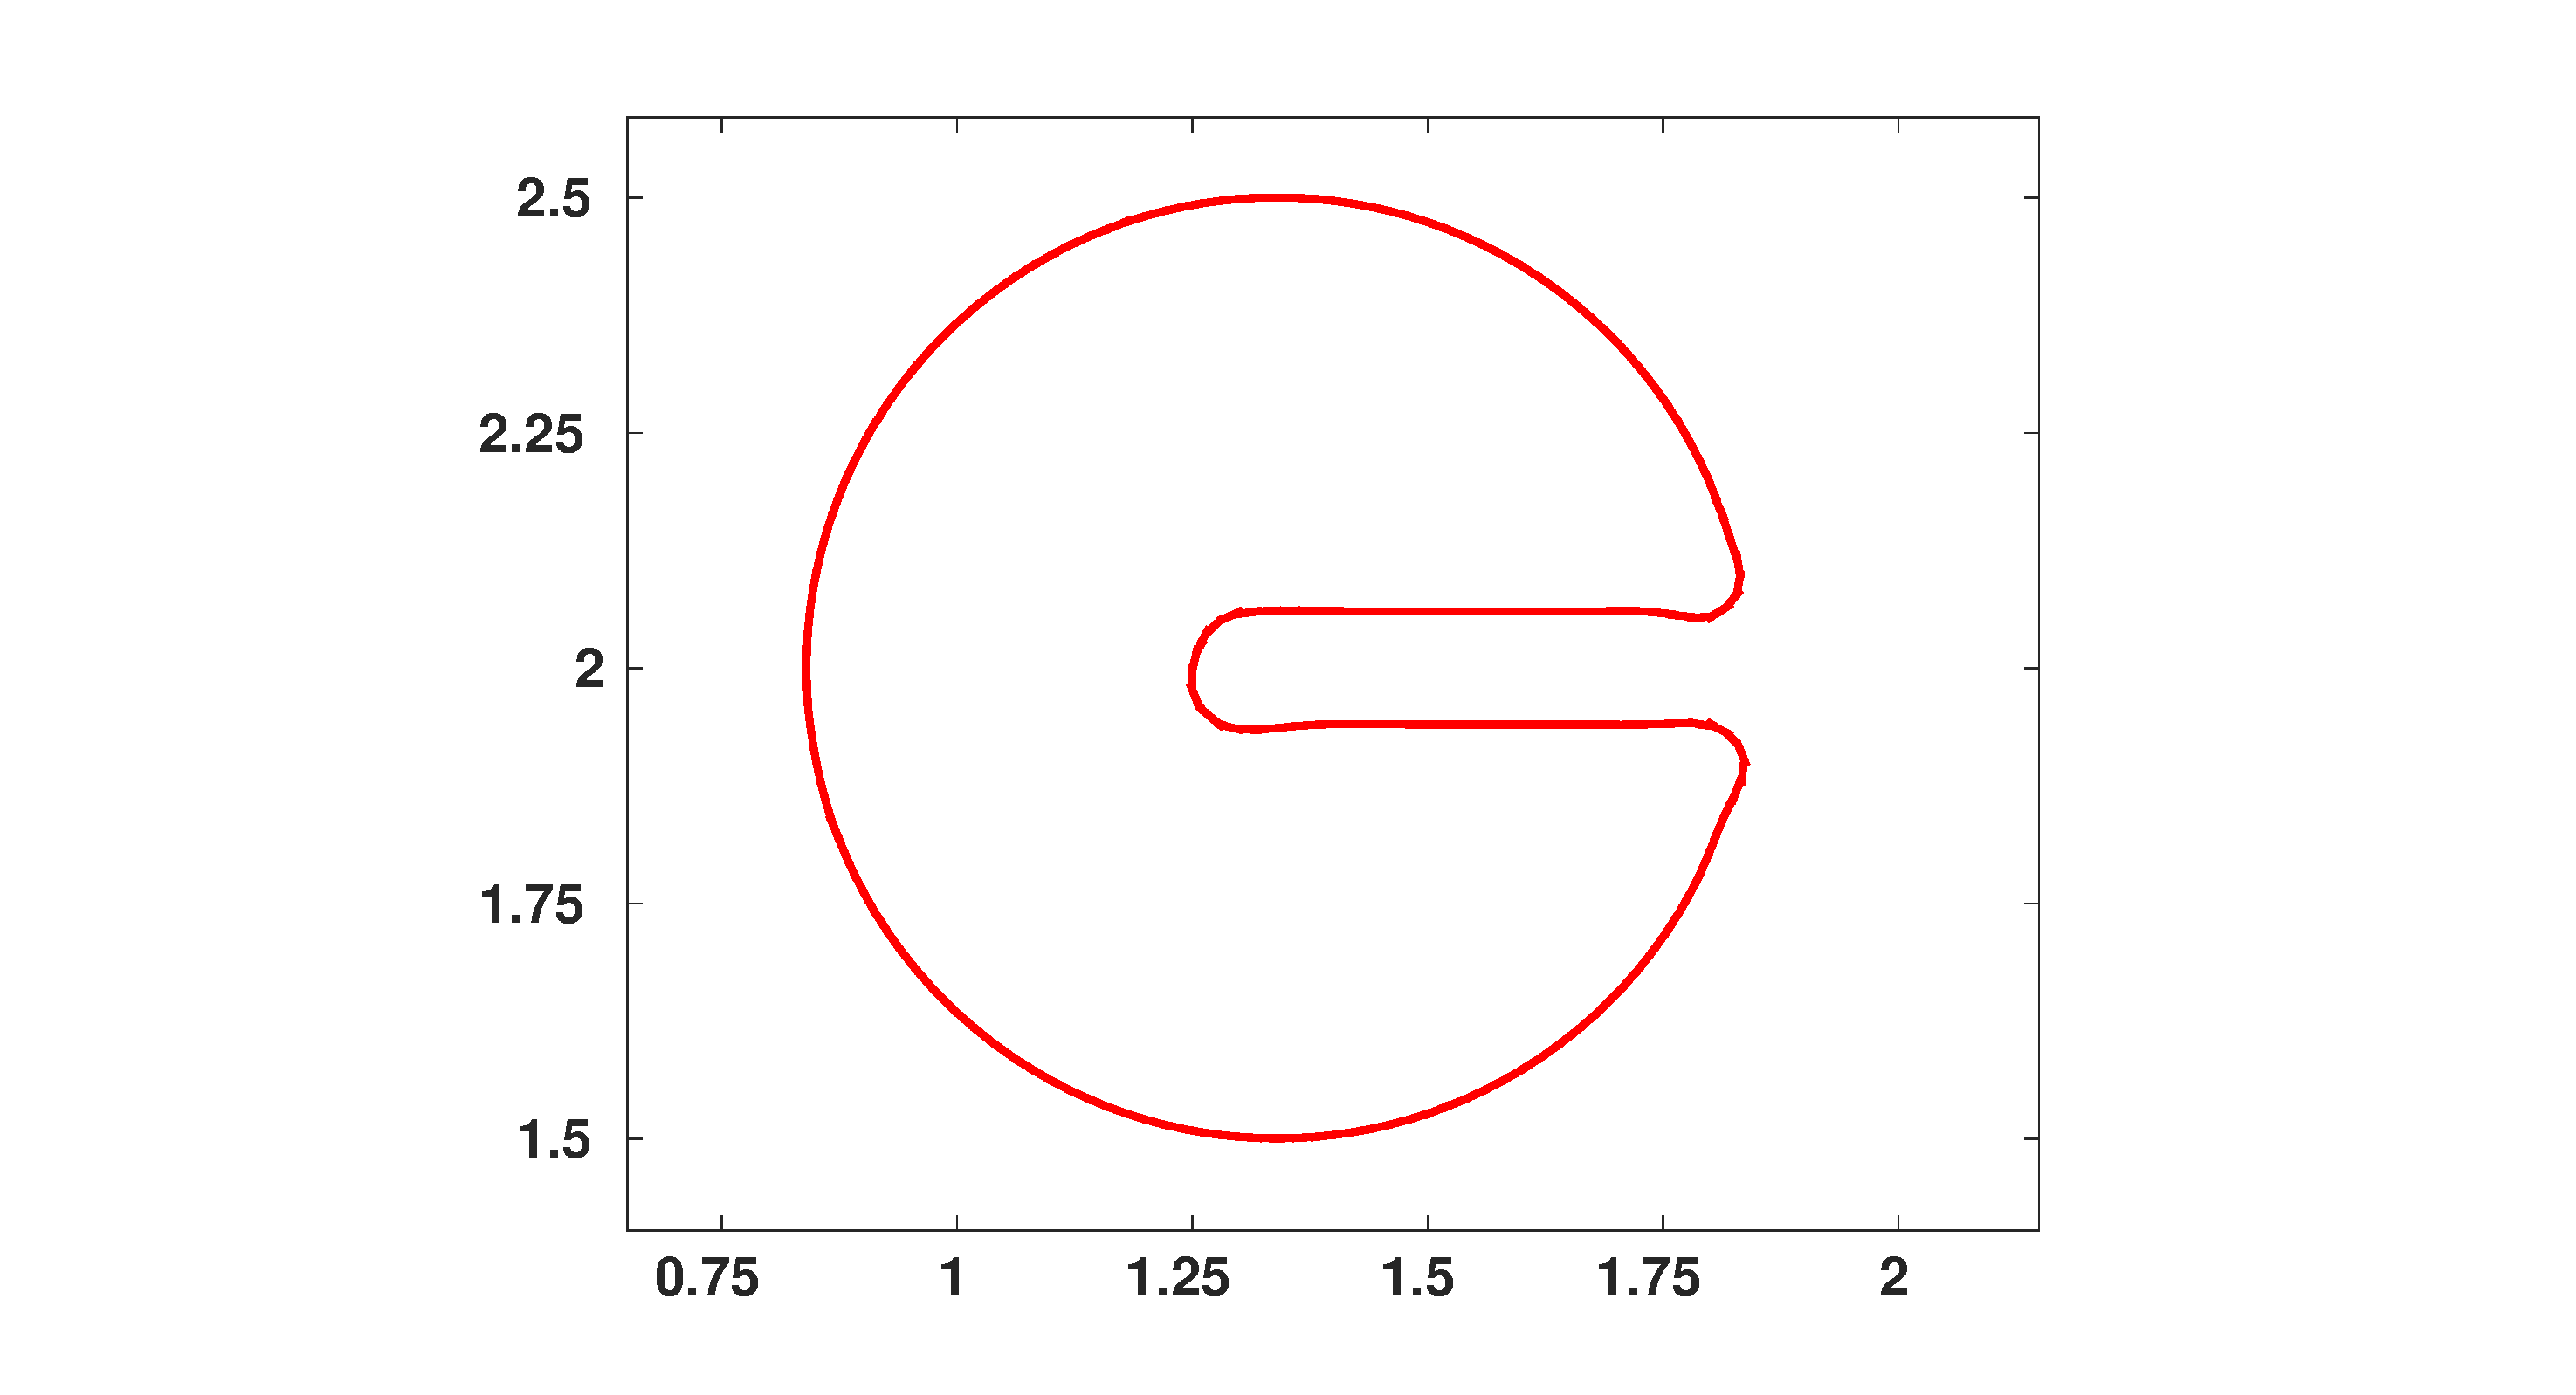
\includegraphics[width=0.5\textwidth]{SC_628.eps}
      }
     \subfloat[After advecting 1256 steps\label{subfig-1:dummy}]{%
      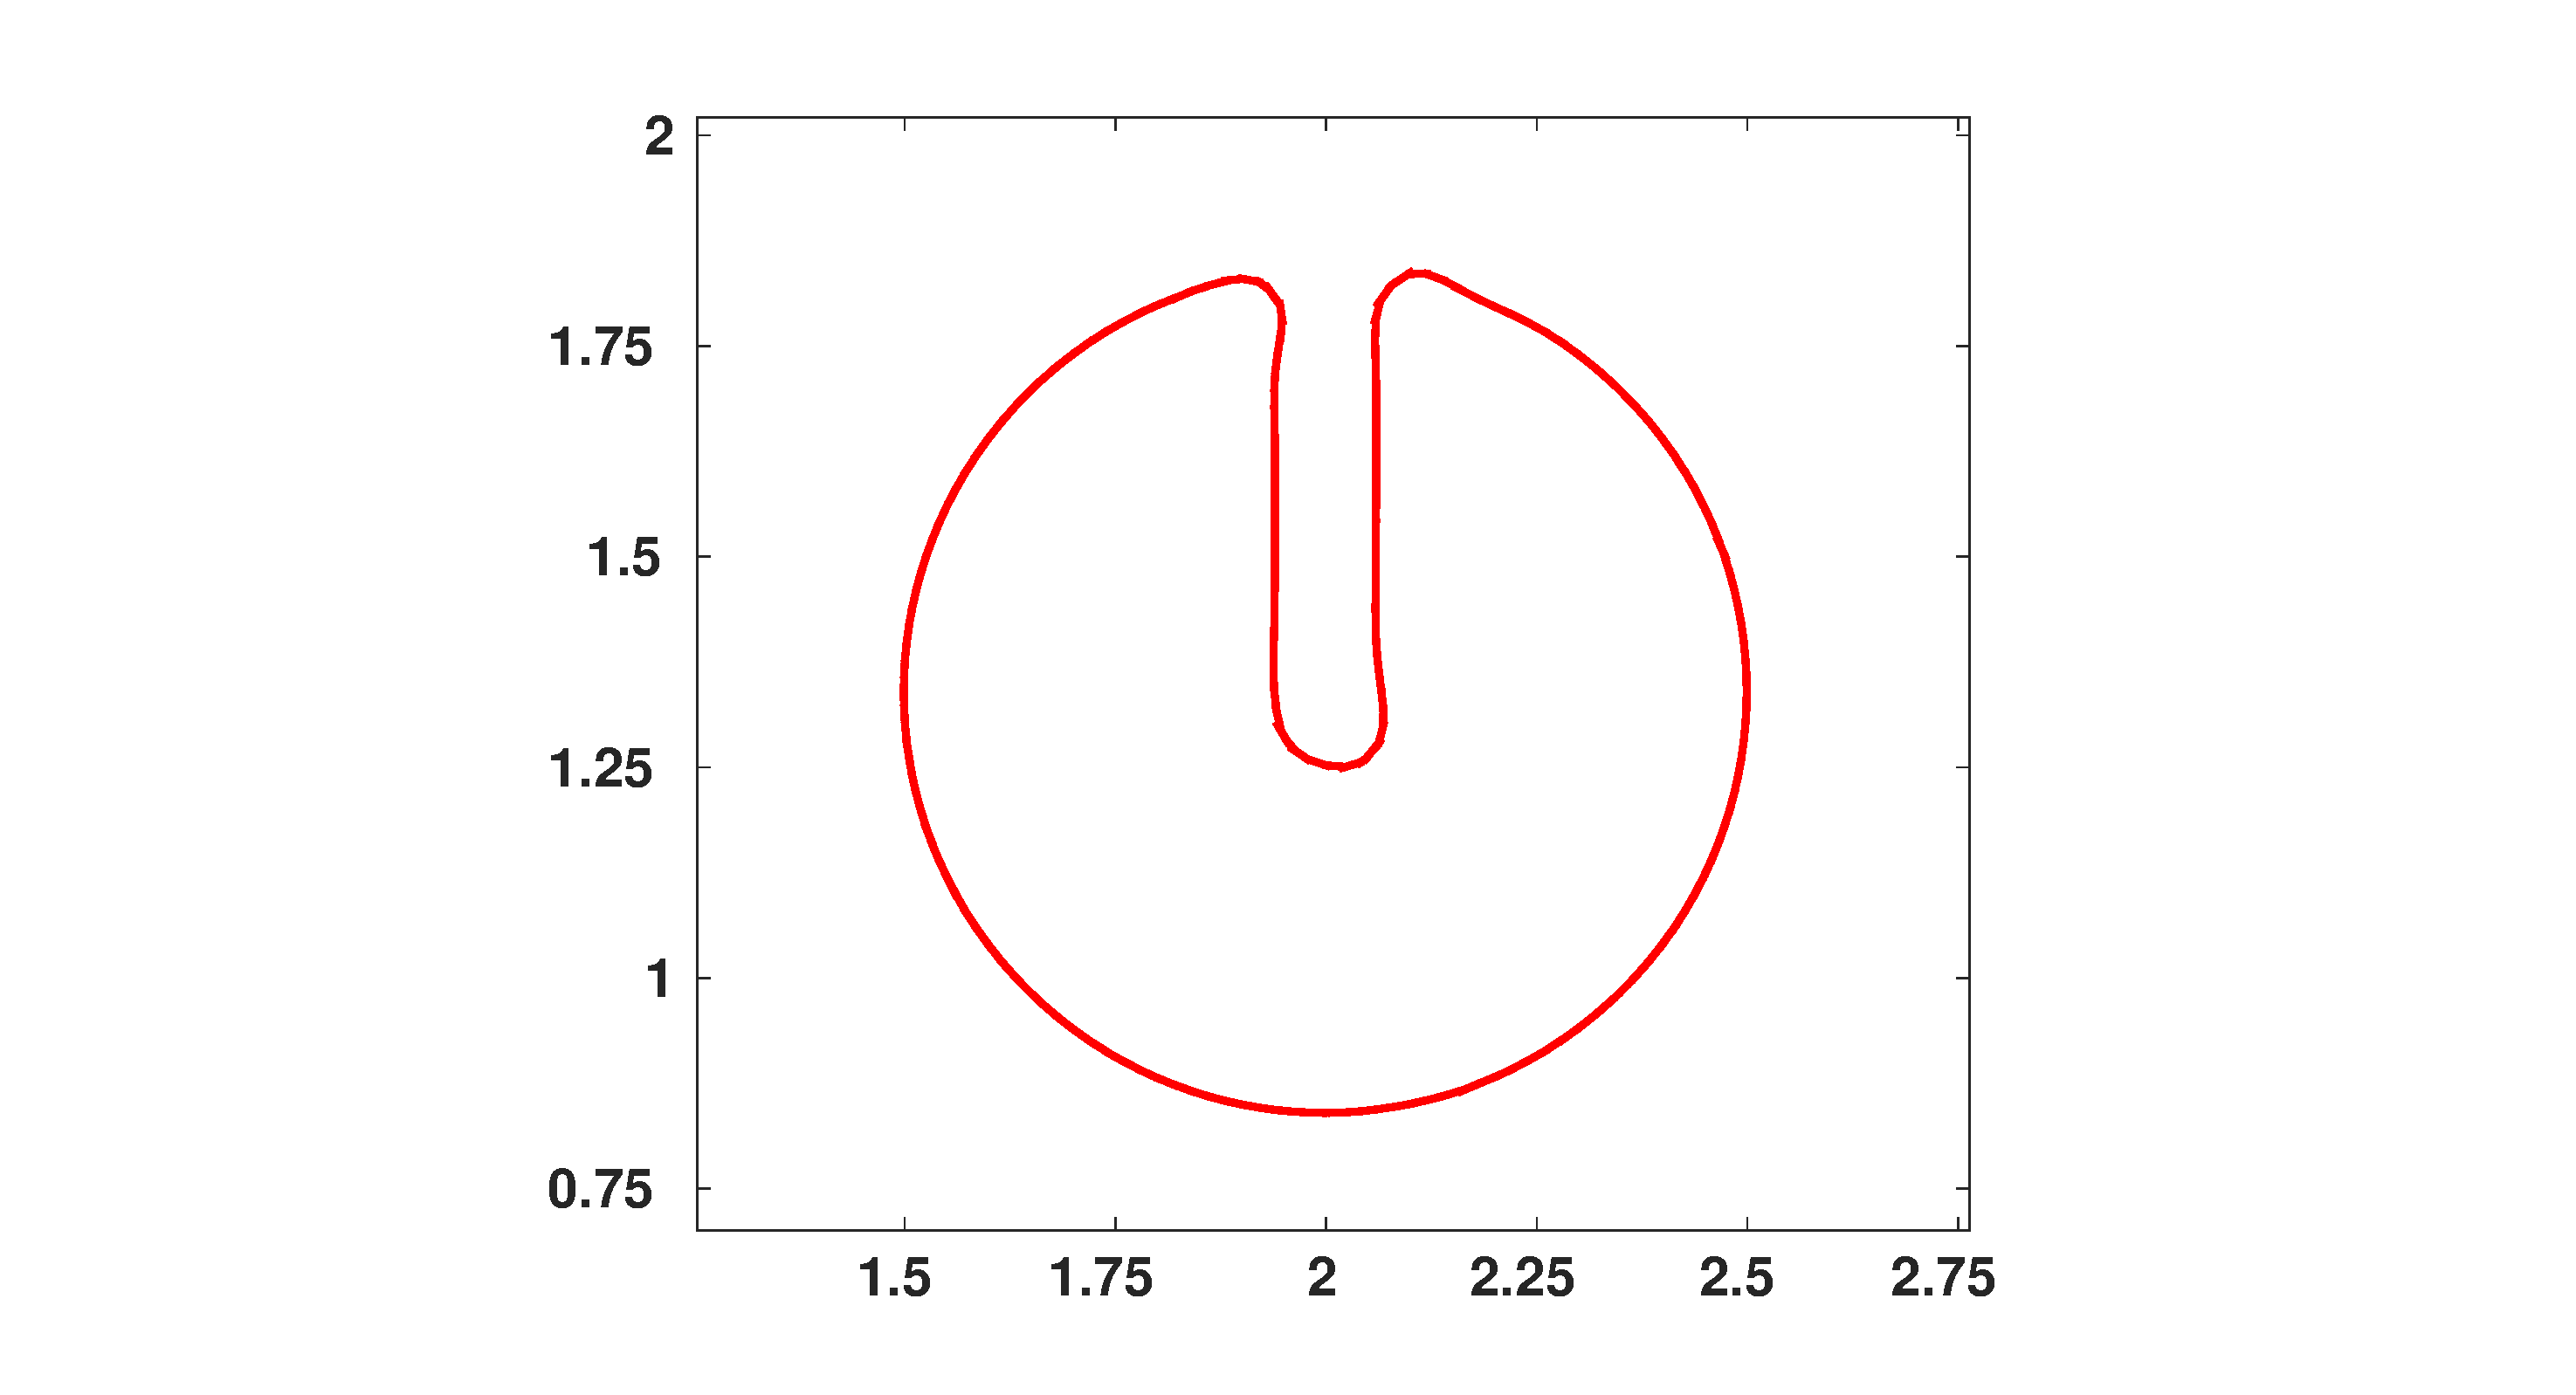
\includegraphics[width=0.5\textwidth]{SC_1256.eps}
      }\\
        \subfloat[After advecting 1885 steps\label{subfig-1:dummy}]{%
      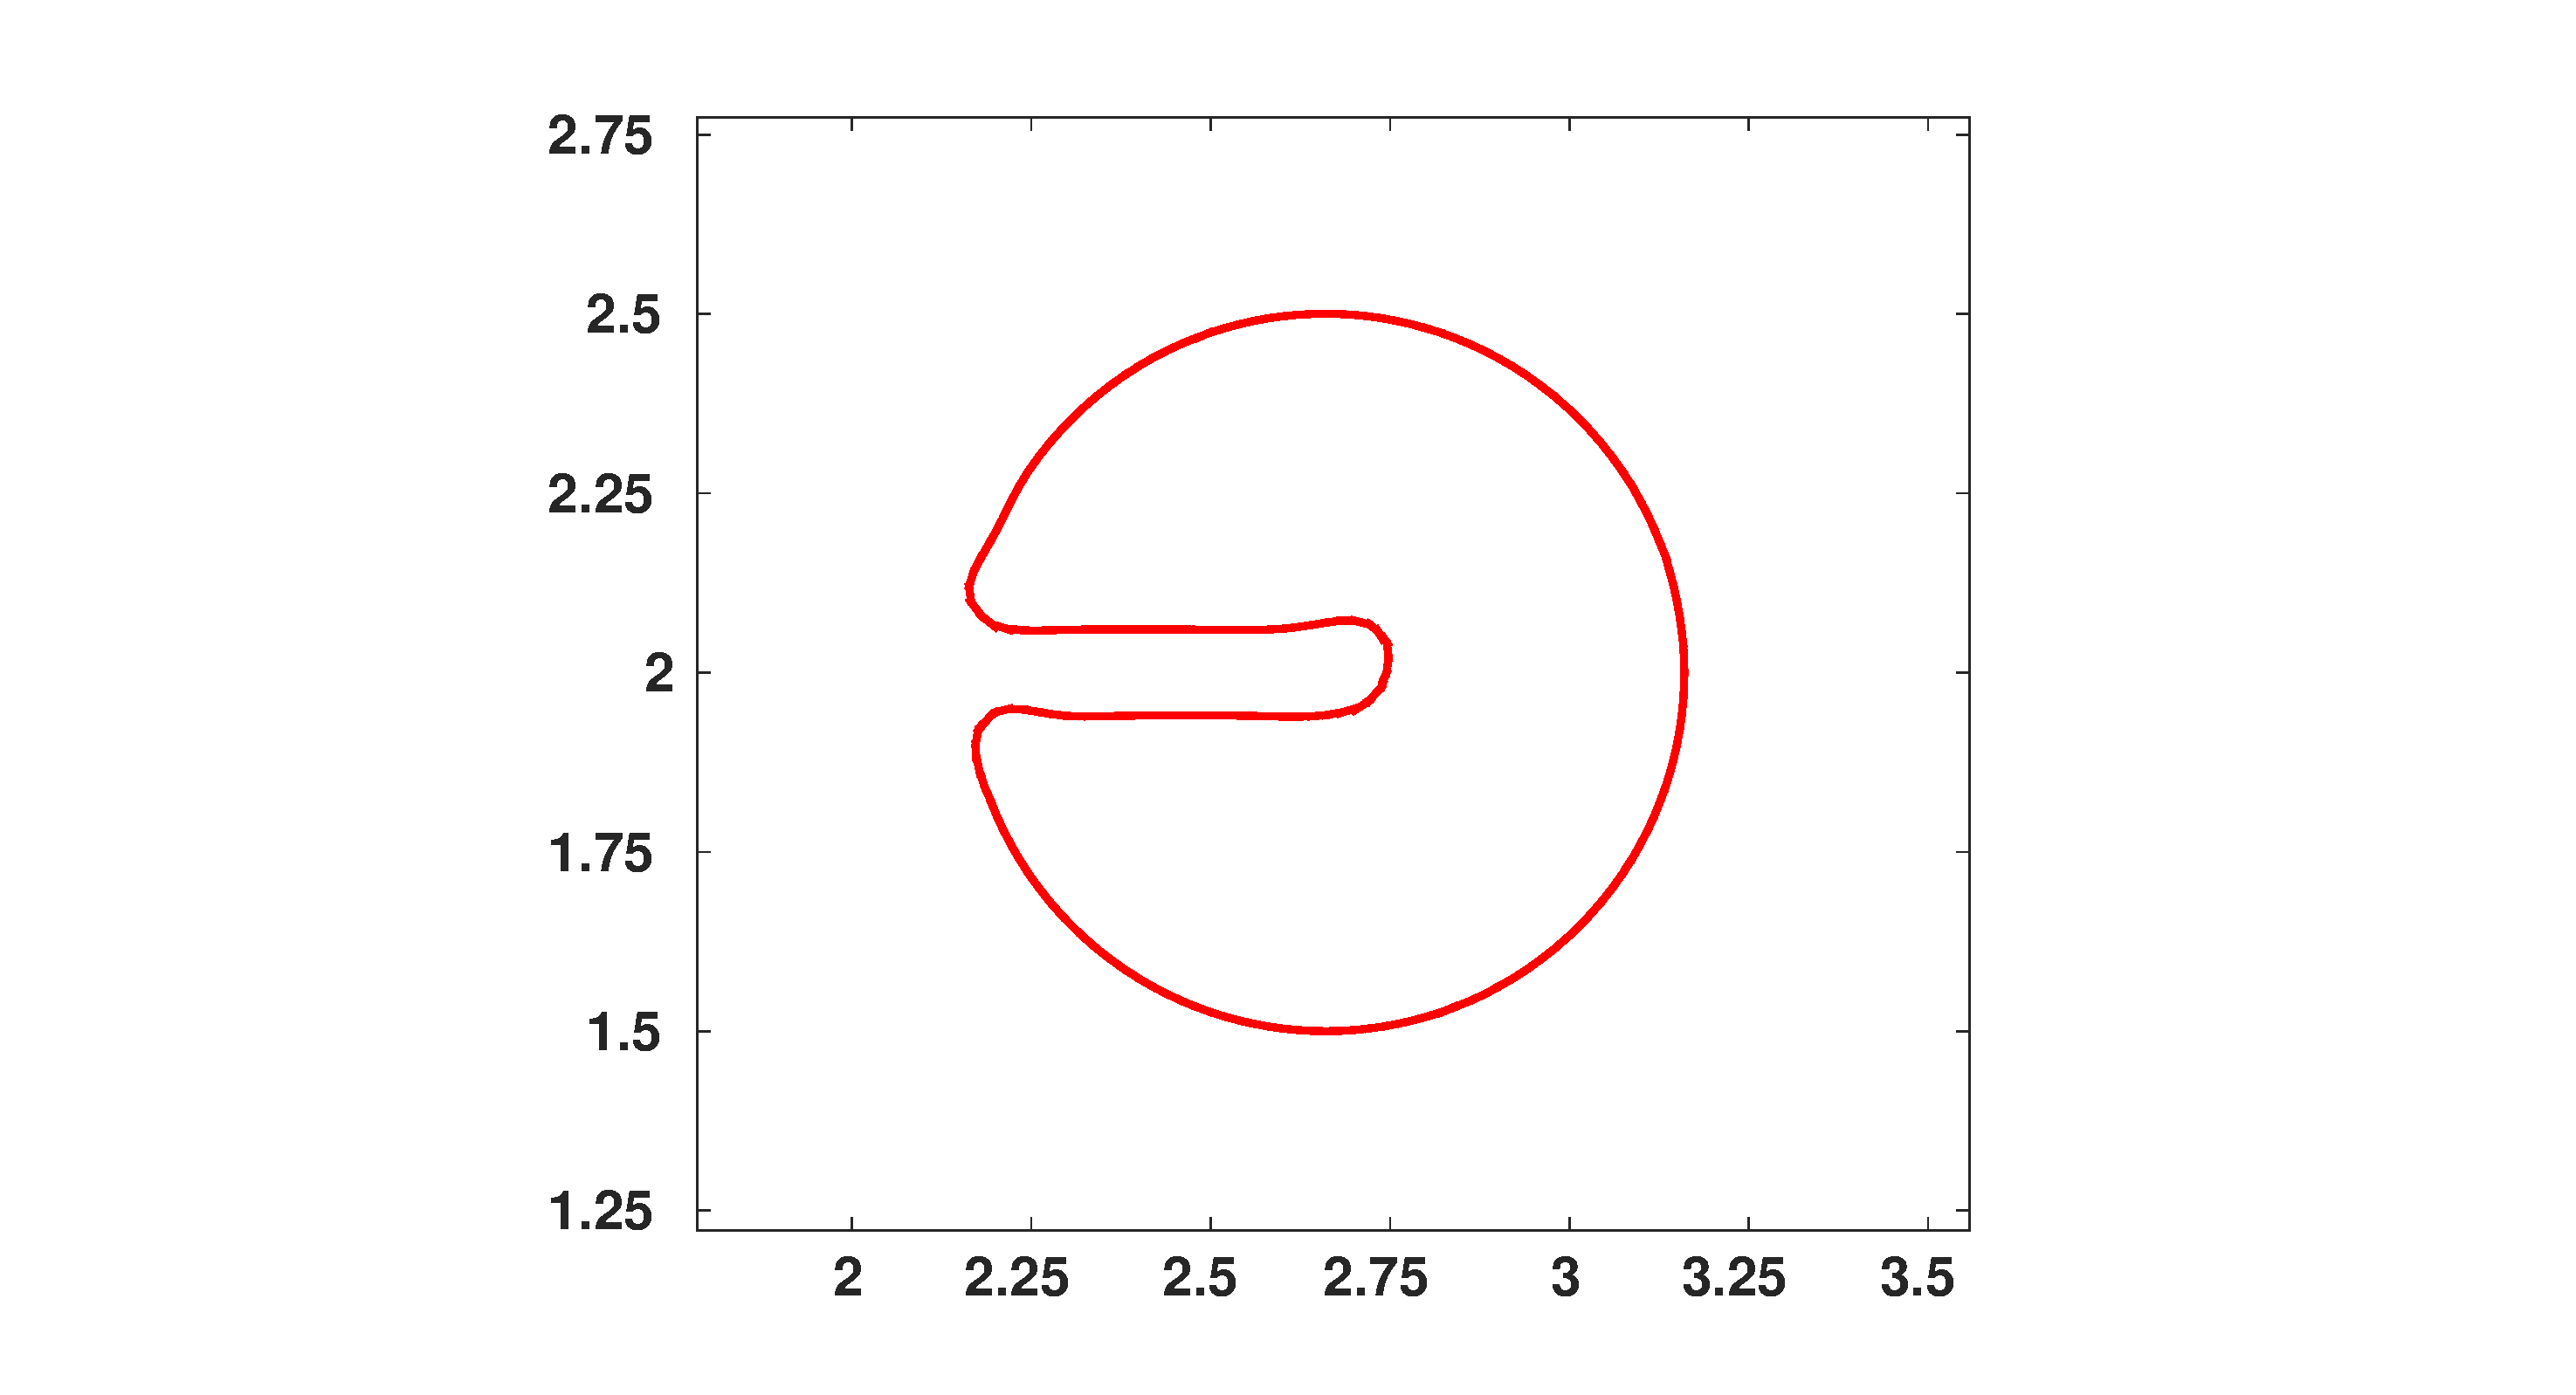
\includegraphics[width=0.5\textwidth]{SC_1885.eps}
      }
        \subfloat[After advecting 2513 steps\label{subfig-1:dummy}]{%
      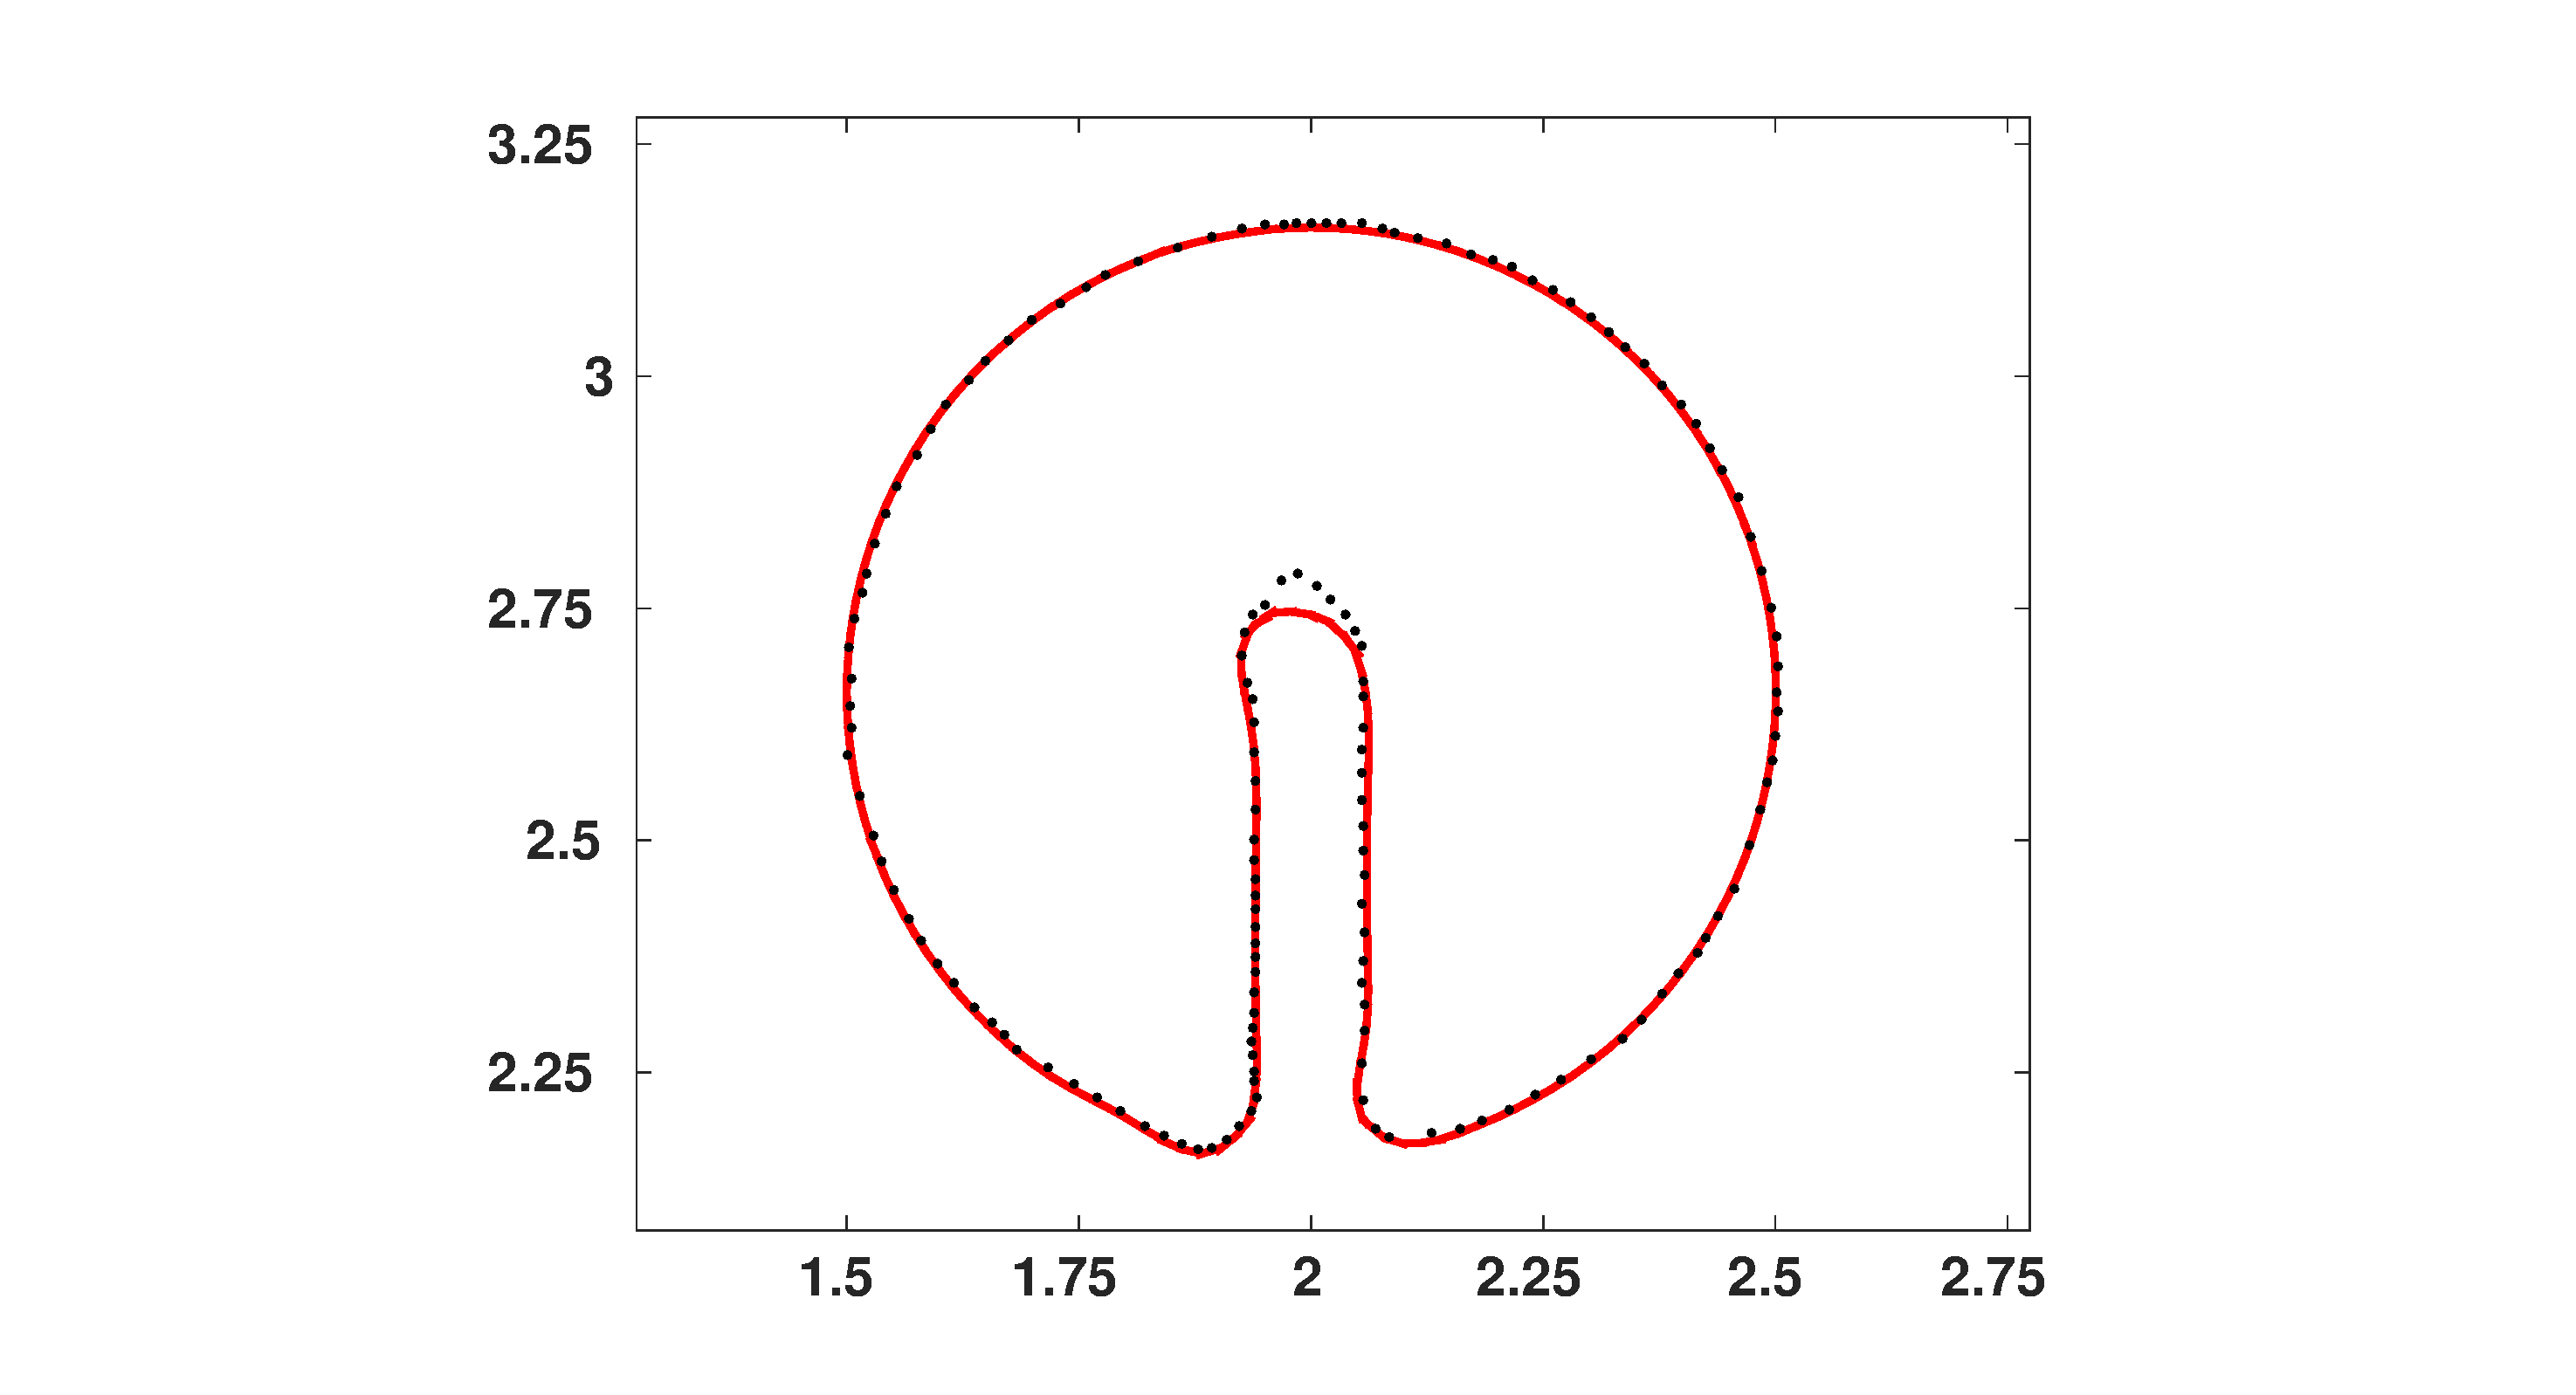
\includegraphics[width=0.5\textwidth]{SC_2513.eps}
      }
 \caption{Advection test result for solid body rotation}
\end{figure}
% 
\subsection{Shear Test}
The real problems typically encounters the interface deformation, which includes merging and deformation. Hence the algorithm has to be 
tested for shear velocity field. The shear test problem verified with \cite{Gerlach2006}. 

   \begin{enumerate}
 \item Domain: [0,$\pi$] x [0,$\pi$]
 \item Grid Size: 100 x 100
 \item Radius of circle :$\frac{pi}{5}$
 \item Center : $(\pi/2,\pi/4)$
 \item Velocity field(Forward):  $U(sin x cos y, -cos x sin y)$
  \item Velocity field(Backward):  $U(-sin x cos y, cos x sin y)$
 \end{enumerate}
 
\begin{figure}[H]
\centering
   \subfloat[Initial condition for shear test\label{subfig-1:dummy}]{%
      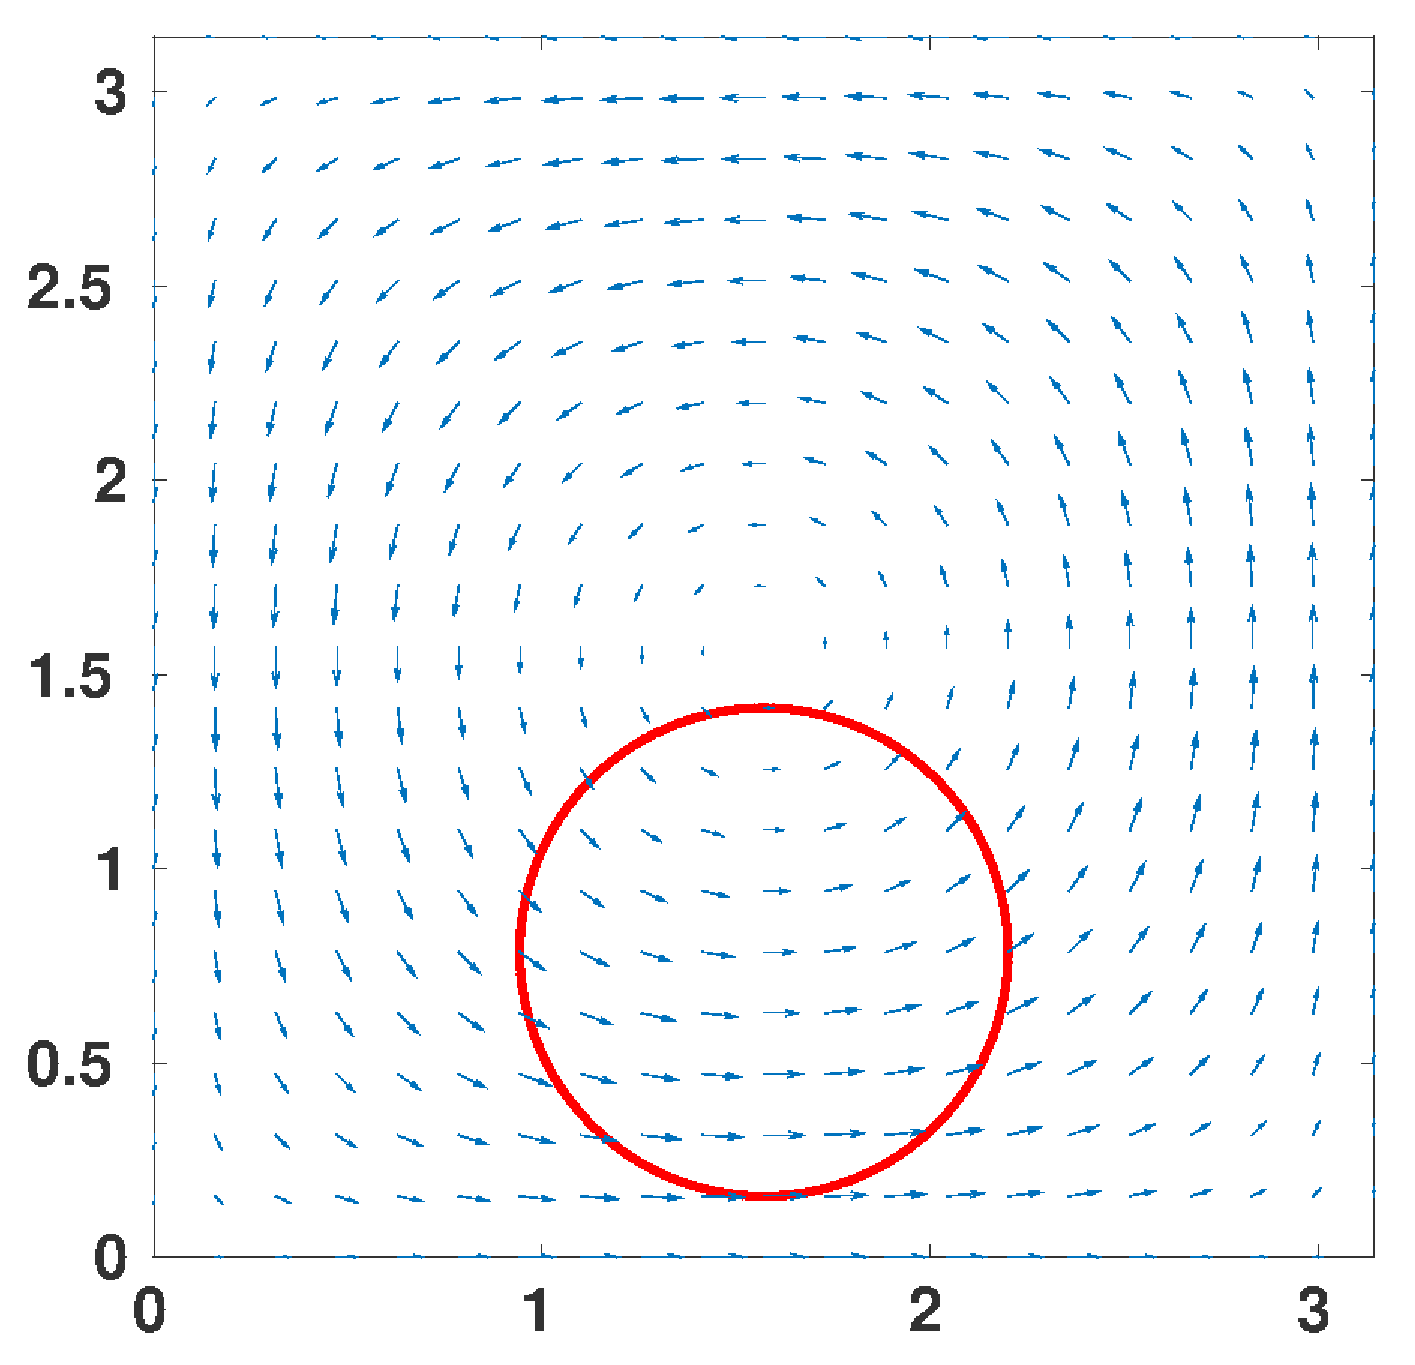
\includegraphics[width=0.5\textwidth]{shear_IC.eps}
      }
\subfloat[After advecting 250 steps\label{subfig-1:dummy}]{%
      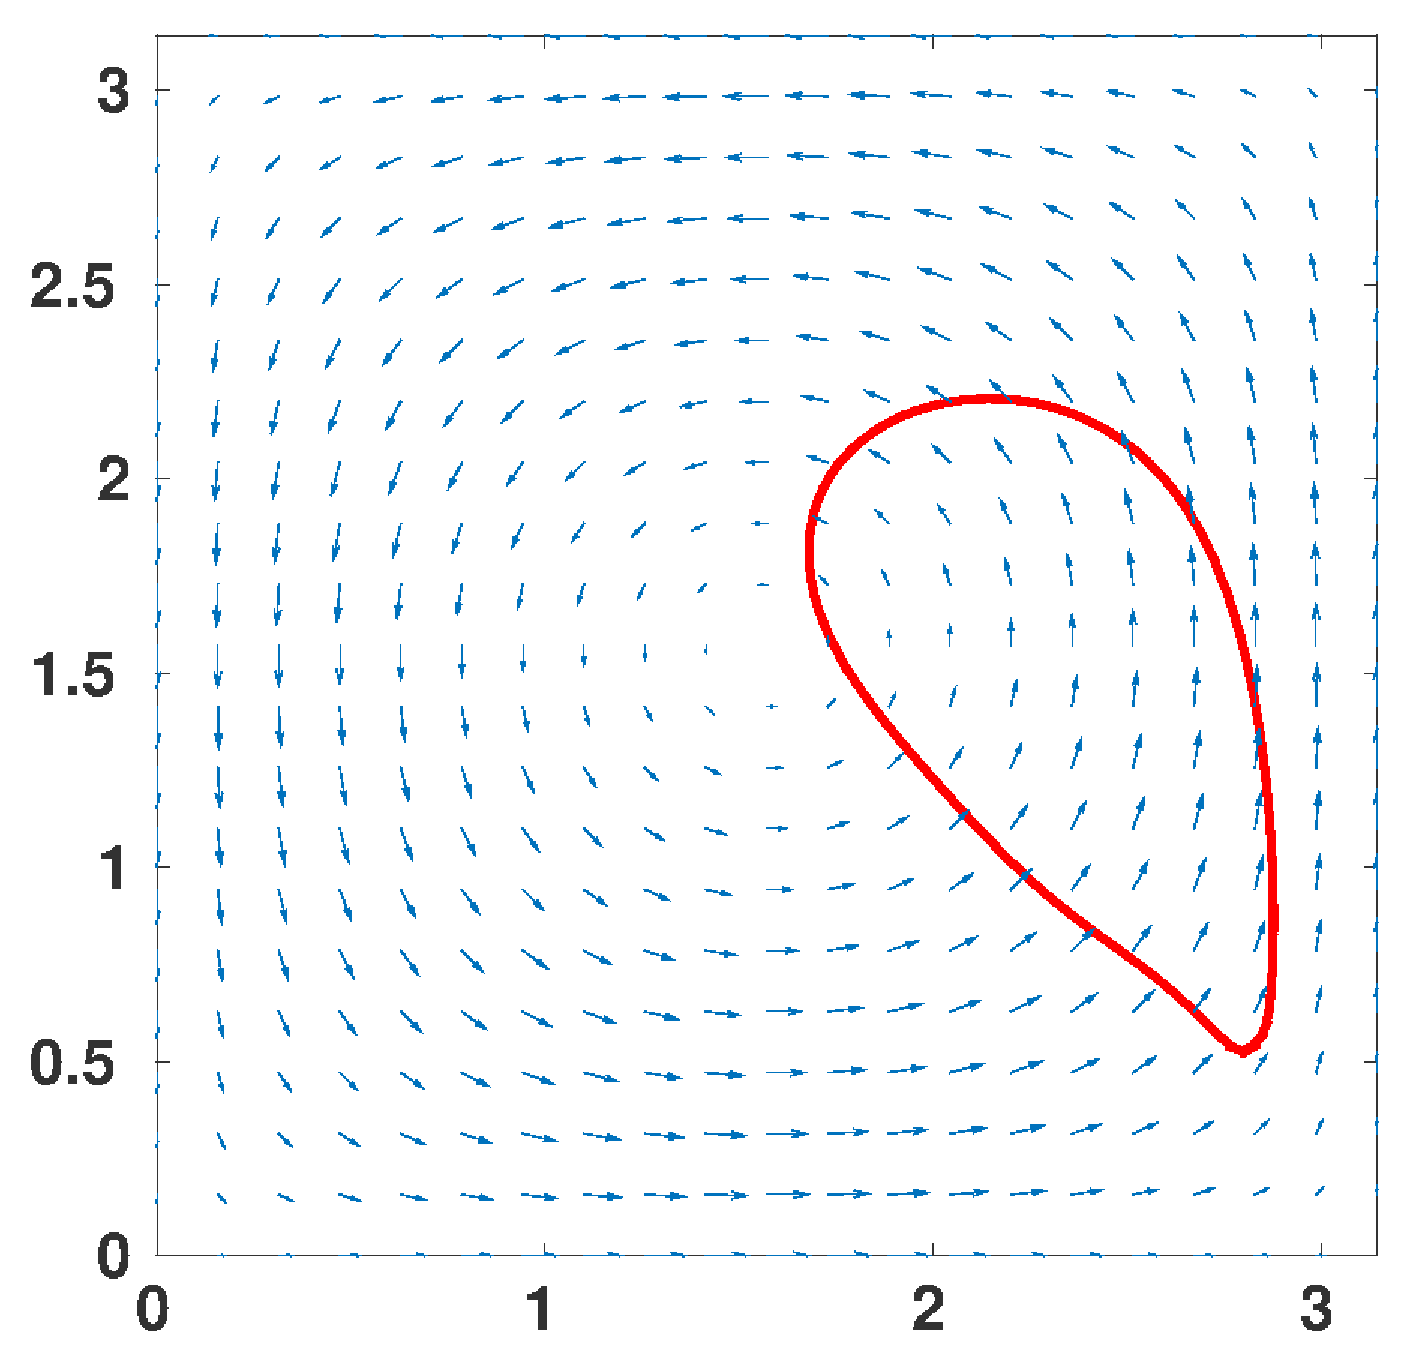
\includegraphics[width=0.5\textwidth]{shear_250.eps}
      } \\
      \subfloat[After advecting 500 steps\label{subfig-1:dummy}]{%
      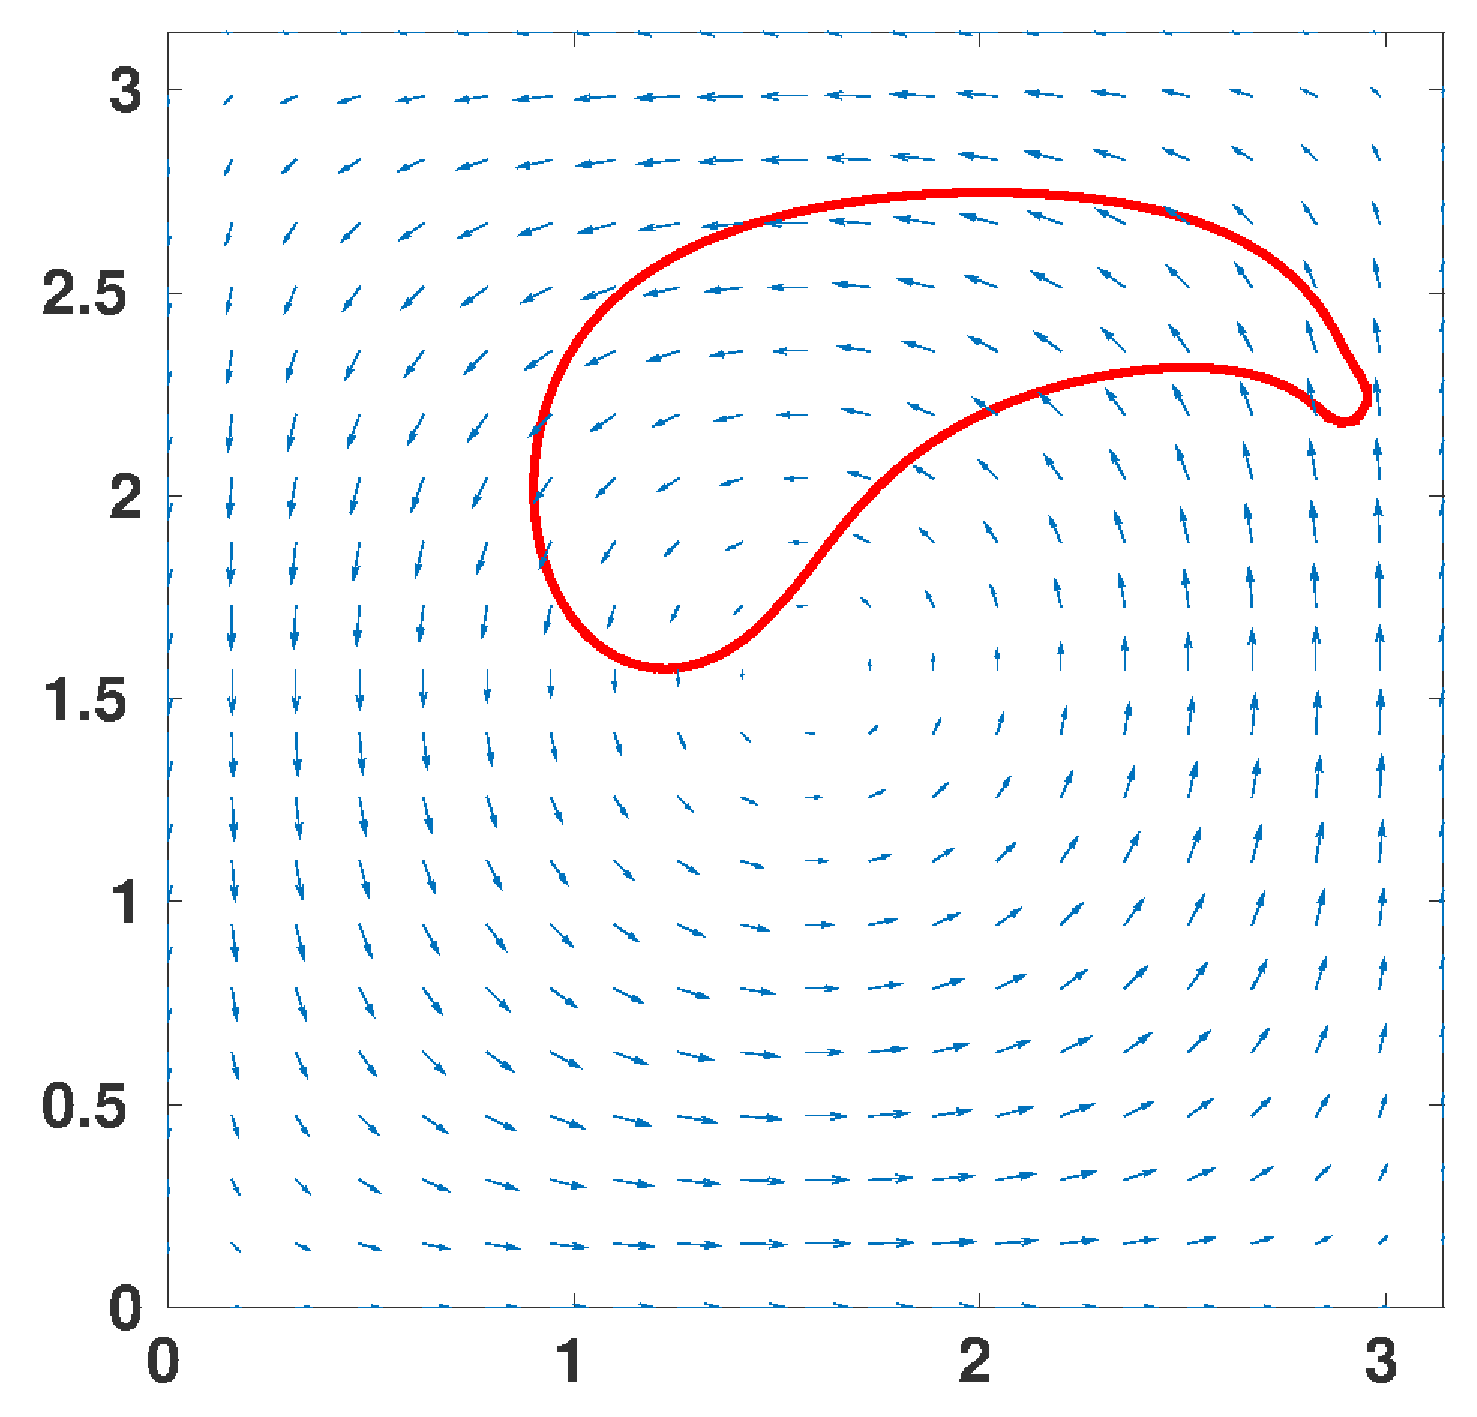
\includegraphics[width=0.5\textwidth]{shear_500.eps}
      }
      \subfloat[After advecting 1000 steps\label{subfig-1:dummy}]{%
      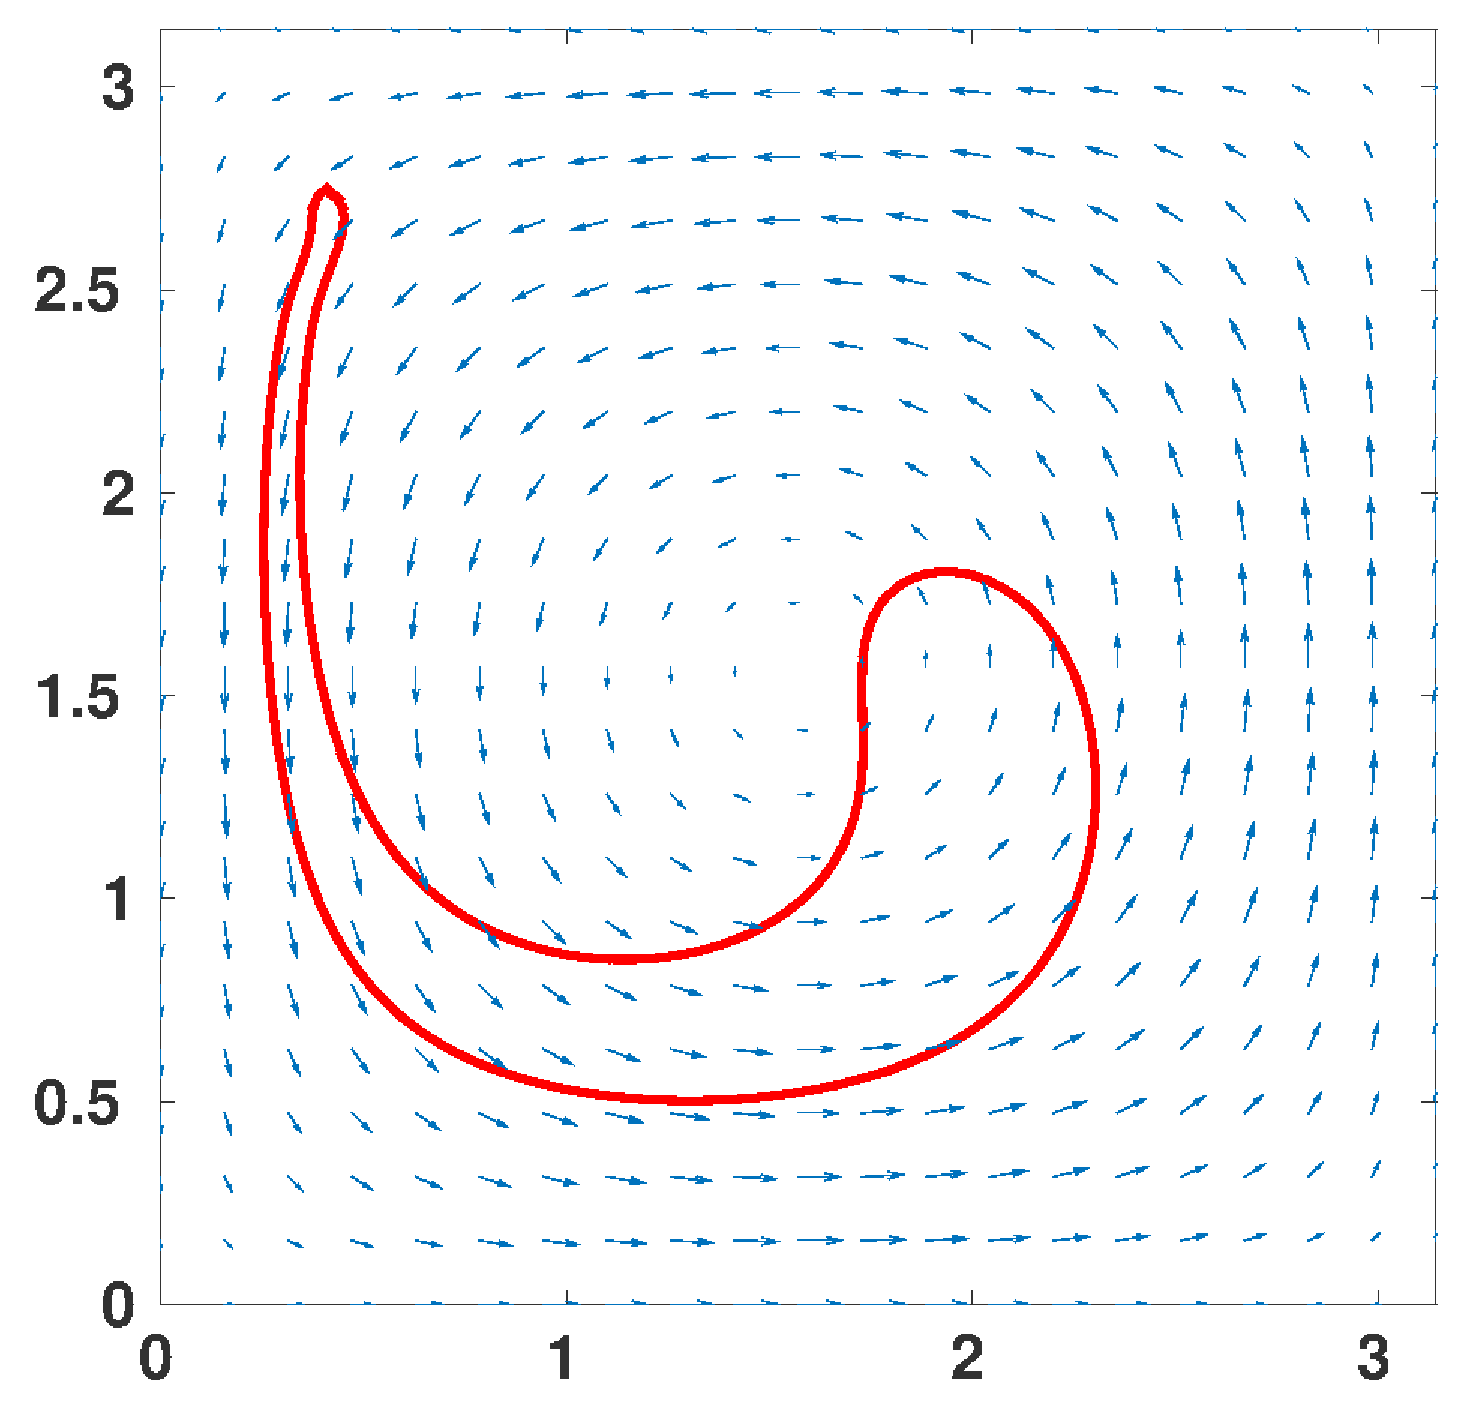
\includegraphics[width=0.5\textwidth]{shear_1000.eps}
      }
 \caption{Advection test result for shear velocity field}
\end{figure}

\begin{figure}[H]
 \centering
 \subfloat[After 1000 steps forward\label{subfig-1:dummy}]{%
      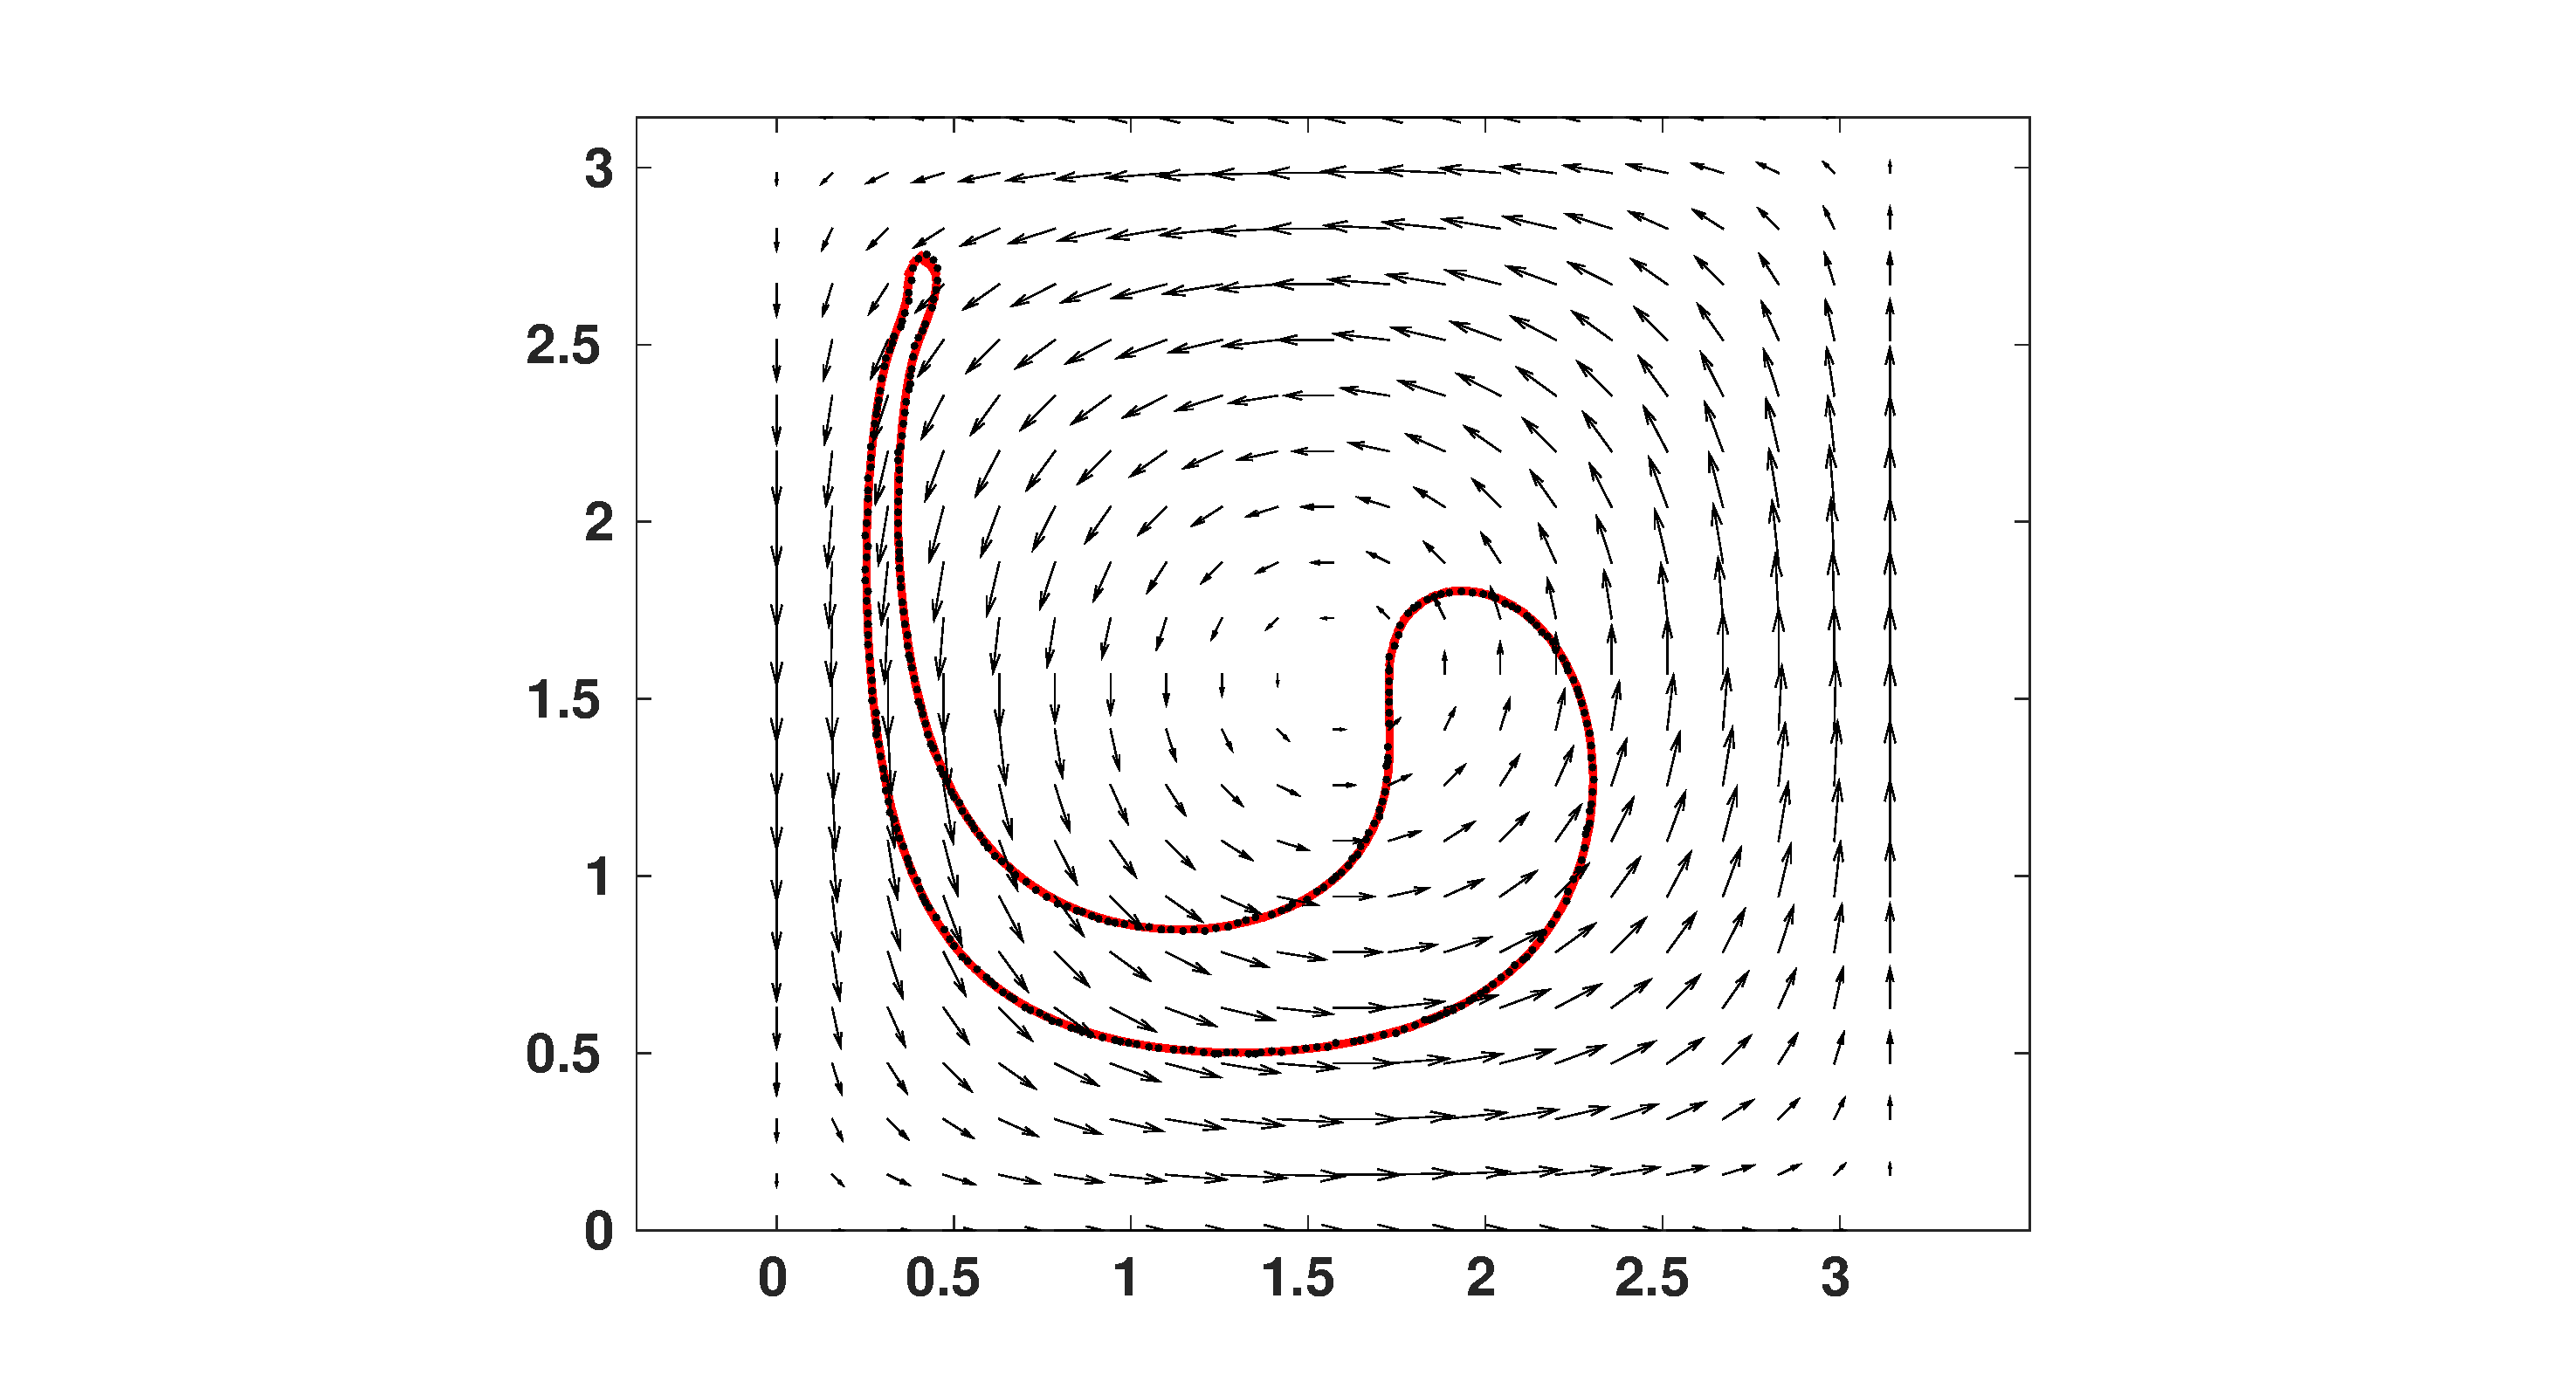
\includegraphics[width=0.5\textwidth]{shear_1000c.eps}
      }
  \subfloat[1000 steps backward followed by 1000 steps forward\label{subfig-1:dummy}]{%
      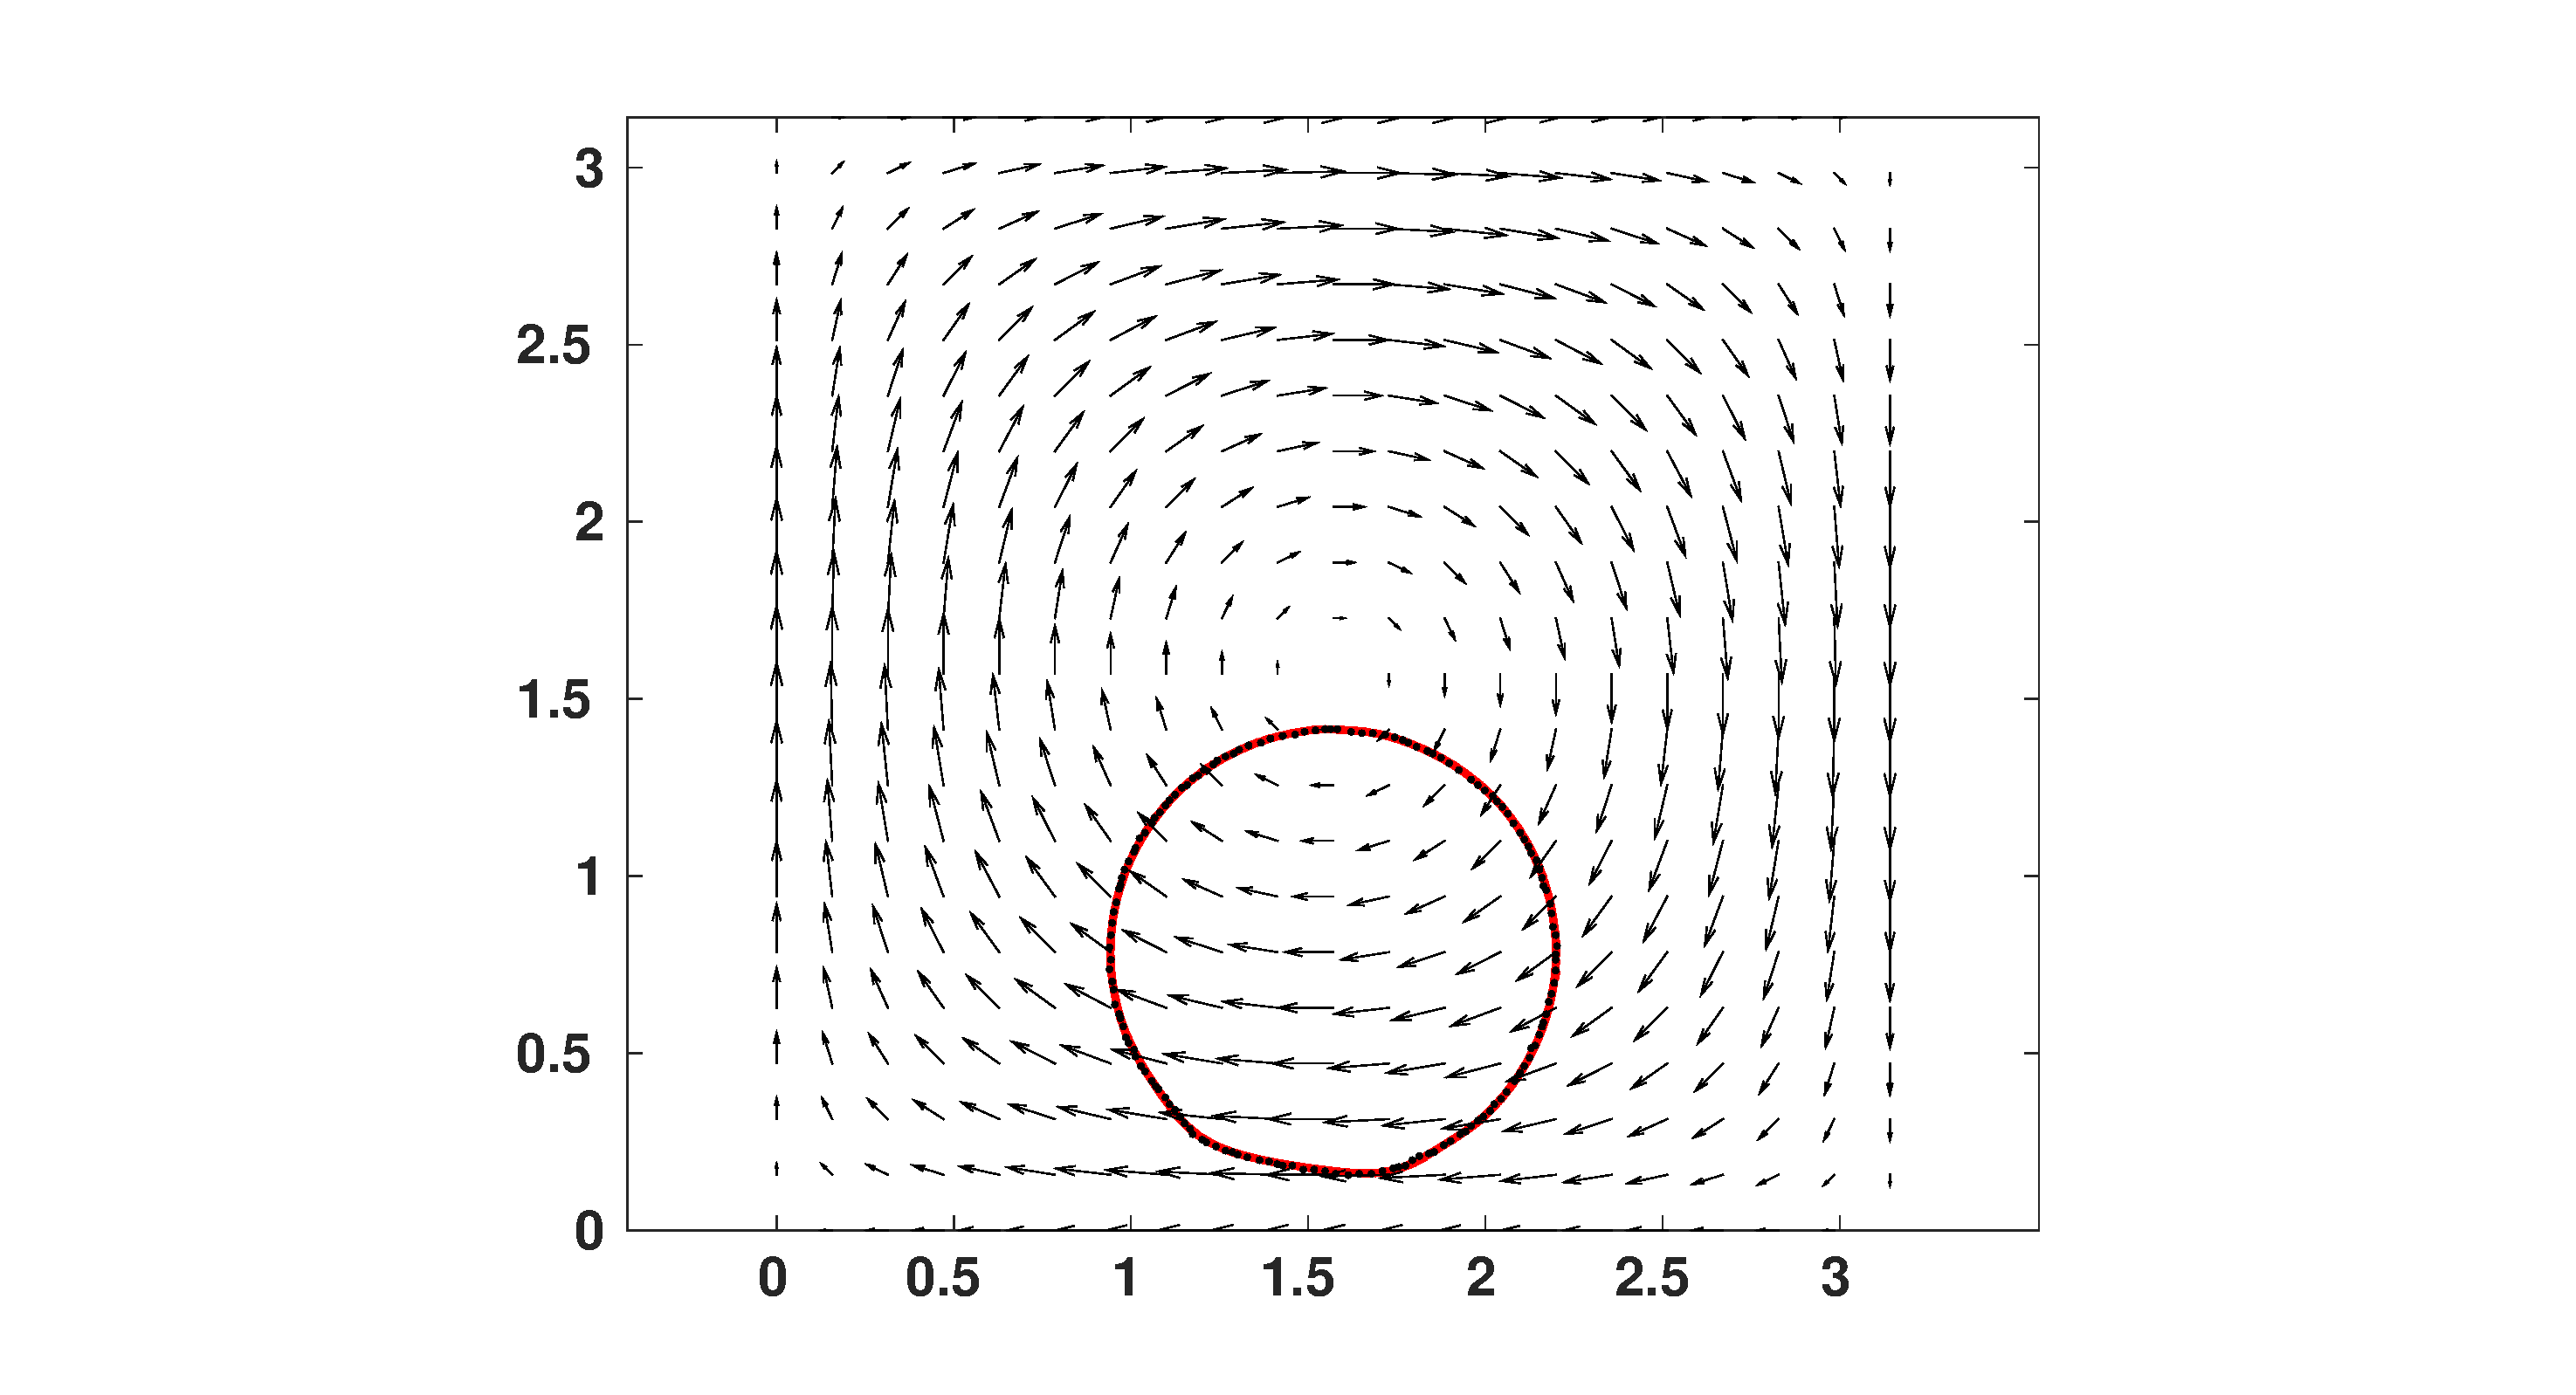
\includegraphics[width=0.5\textwidth]{shear_back.eps}
      }
 \caption{Comparison with \cite{Gerlach2006} results. (Red LVIRA and Black \cite{Gerlach2006} data)}
\end{figure}

\subsection{Calculation of error}
The above results can be quantified by defining the error by
\begin{equation}
 E = \frac{\sum |{V^n_{i,j}-V^e_{i,j}}|}{\sum V^0_{i,j}}
\end{equation}

where $V^n$ is the solution of volume fraction field after n time steps by computation, $V^e$ is the exact solution, and $V^0$ is the initial solution. The initial solution can be calculated by the initial 
volume fraction field, exact solution of fields for translational fields can be easily calculated by recreating the circle at the center which has moved with the velocity field. For solid body
rotation the exact solution is equals to the initial solution after one full rotation. For shear after 1000 backward steps the final solution should also be equal to initial solution.

\begin{table}[H]
  \begin{center}
    \caption{Error for various tests}
    \label{tab:samtab}
    \begin{tabular}{p{3cm}lllll}
      \toprule 
       Test & SLIC & Hirt-Nichols & FCT-VOF & Youngs & LVIRA  \\ 
      \midrule
      Translational (V(1,0)) & $1.30 X 10^{-2}$ & $4.55 X 10^{-2}$ & $1.28 X 10^{-2}$ & $3.08 X 10^{-3}$ & $1.5 X 10^{-3}$  \\ 
        Translational (V(2,1)) & $9.18 X 10^{-2}$ & $1.9 X 10^{-1}$ & $3.99 X 10^{-2}$ & $2.98 X 10^{-2}$ & $1.05 X 10^{-2}$  \\ 
      Shear Flow & $4.59 X 10^{-2}$ & $6.66 X 10^{-2}$ & $3.14 X 10^{-2}$ & $8.60 X 10^{-3}$ & $6.90 X 10^{-3}$  \\ 
       Solid Body Rotation (Slotted circle) & $8.38 X 10^{-2}$ & $9.62 X 10^{-2}$ & $3.29 X 10^{-2}$ & $1.09 X 10^{-2}$ & $9.7 X 10^{-3}$  \\ 
        
      \bottomrule \\
    \end{tabular}
  \end{center}
\end{table}


